\chapter{Grafici L2}
\label{app:grafici_L2}

Vengono presentati i grafici relativi alle distanze L2 per i vari modelli e attacchi considerati nello studio al capitolo "6.2 - L2 values".

\section{Advanced Adversarial}
\begin{figure}[H]
    \centering
    \begin{subfigure}[b]{0.45\textwidth}
        \centering
        
\includegraphics[width=\textwidth]{immagini/SWEEP L2/AA_Topologia3D_Qwen_Qwen2.5-7B-Instruct_18.png} 
        \caption{Qwen2.5-7B-Instruct}
    \end{subfigure}
    \hfill 
    \begin{subfigure}[b]{0.45\textwidth}
        \centering
        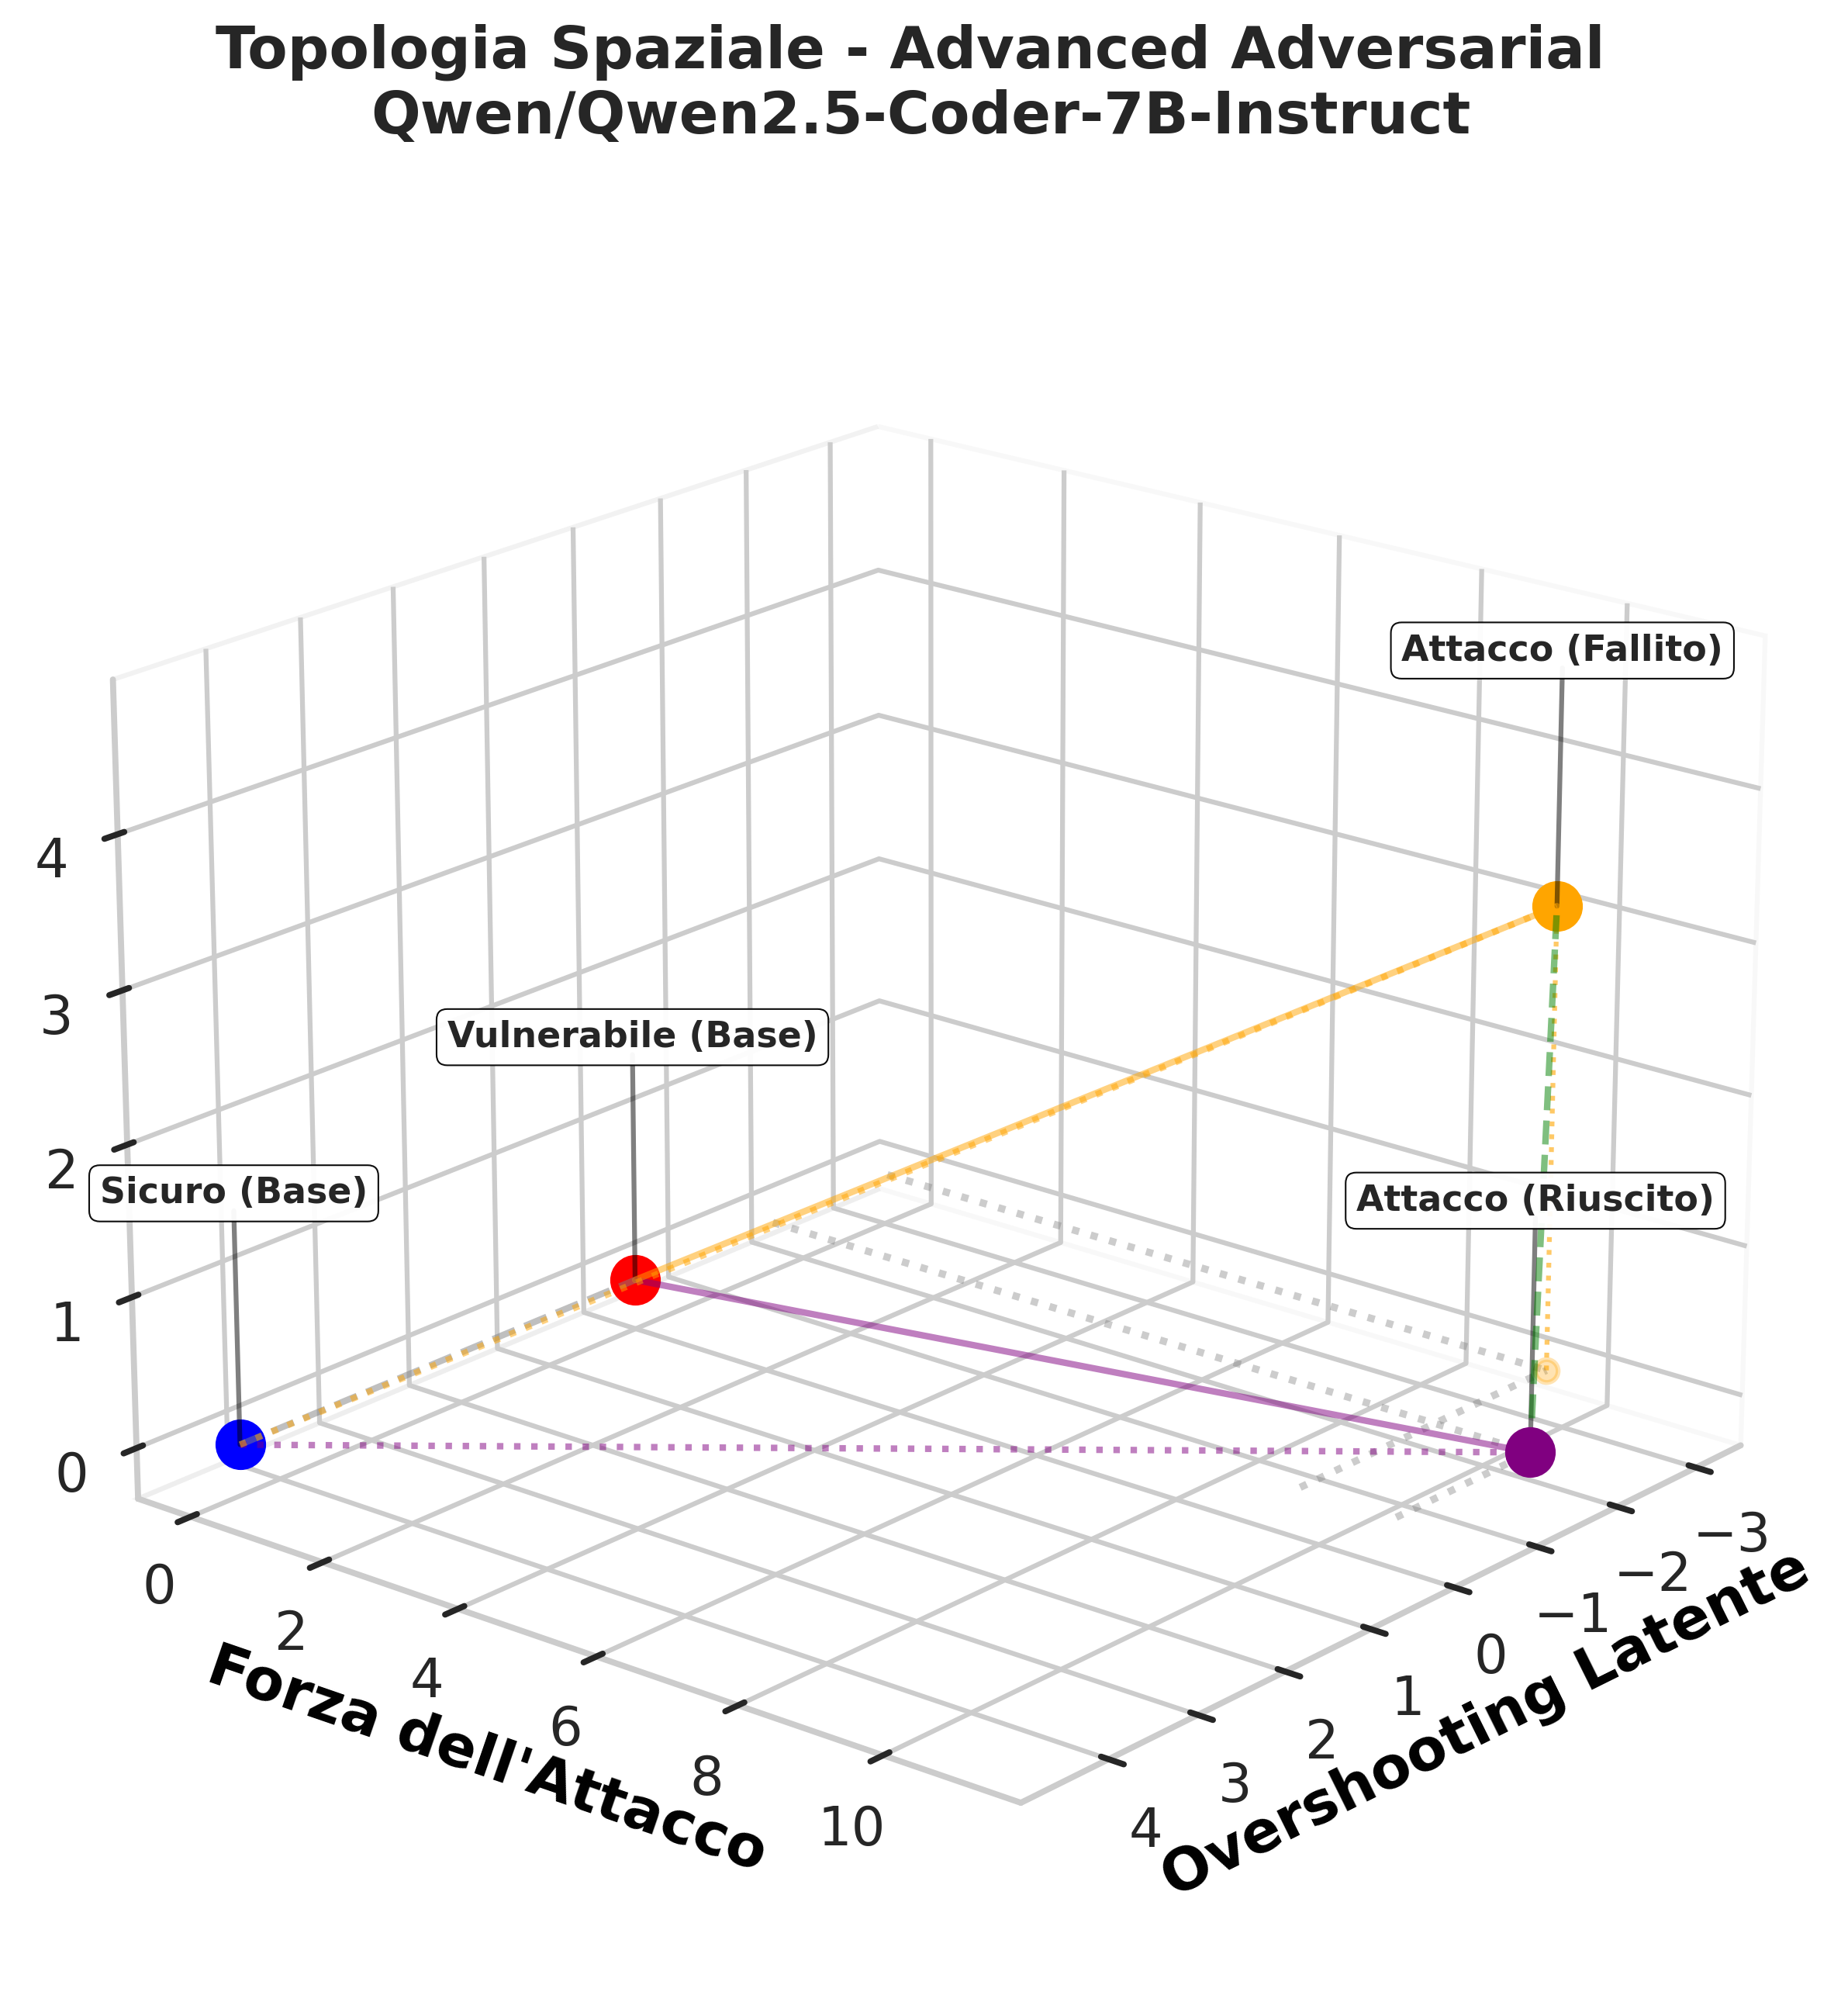
\includegraphics[width=\textwidth]{immagini/SWEEP L2/AA_Topologia3D_Qwen_Qwen2.5-Coder-7B-Instruct_18.png}
        \caption{Qwen2.5-Coder-7B-Instruct}
    \end{subfigure}
\end{figure}

\begin{figure}[H]
    \centering
    \begin{subfigure}[b]{0.45\textwidth}
        \centering
        
\includegraphics[width=\textwidth]{immagini/SWEEP L2/AA_Topologia3D_meta-llama_Llama-3.1-8B-Instruct_15.png} 
        \caption{Llama-3.1-8B-Instruct}
    \end{subfigure}
    \hfill 
    \begin{subfigure}[b]{0.45\textwidth}
        \centering
        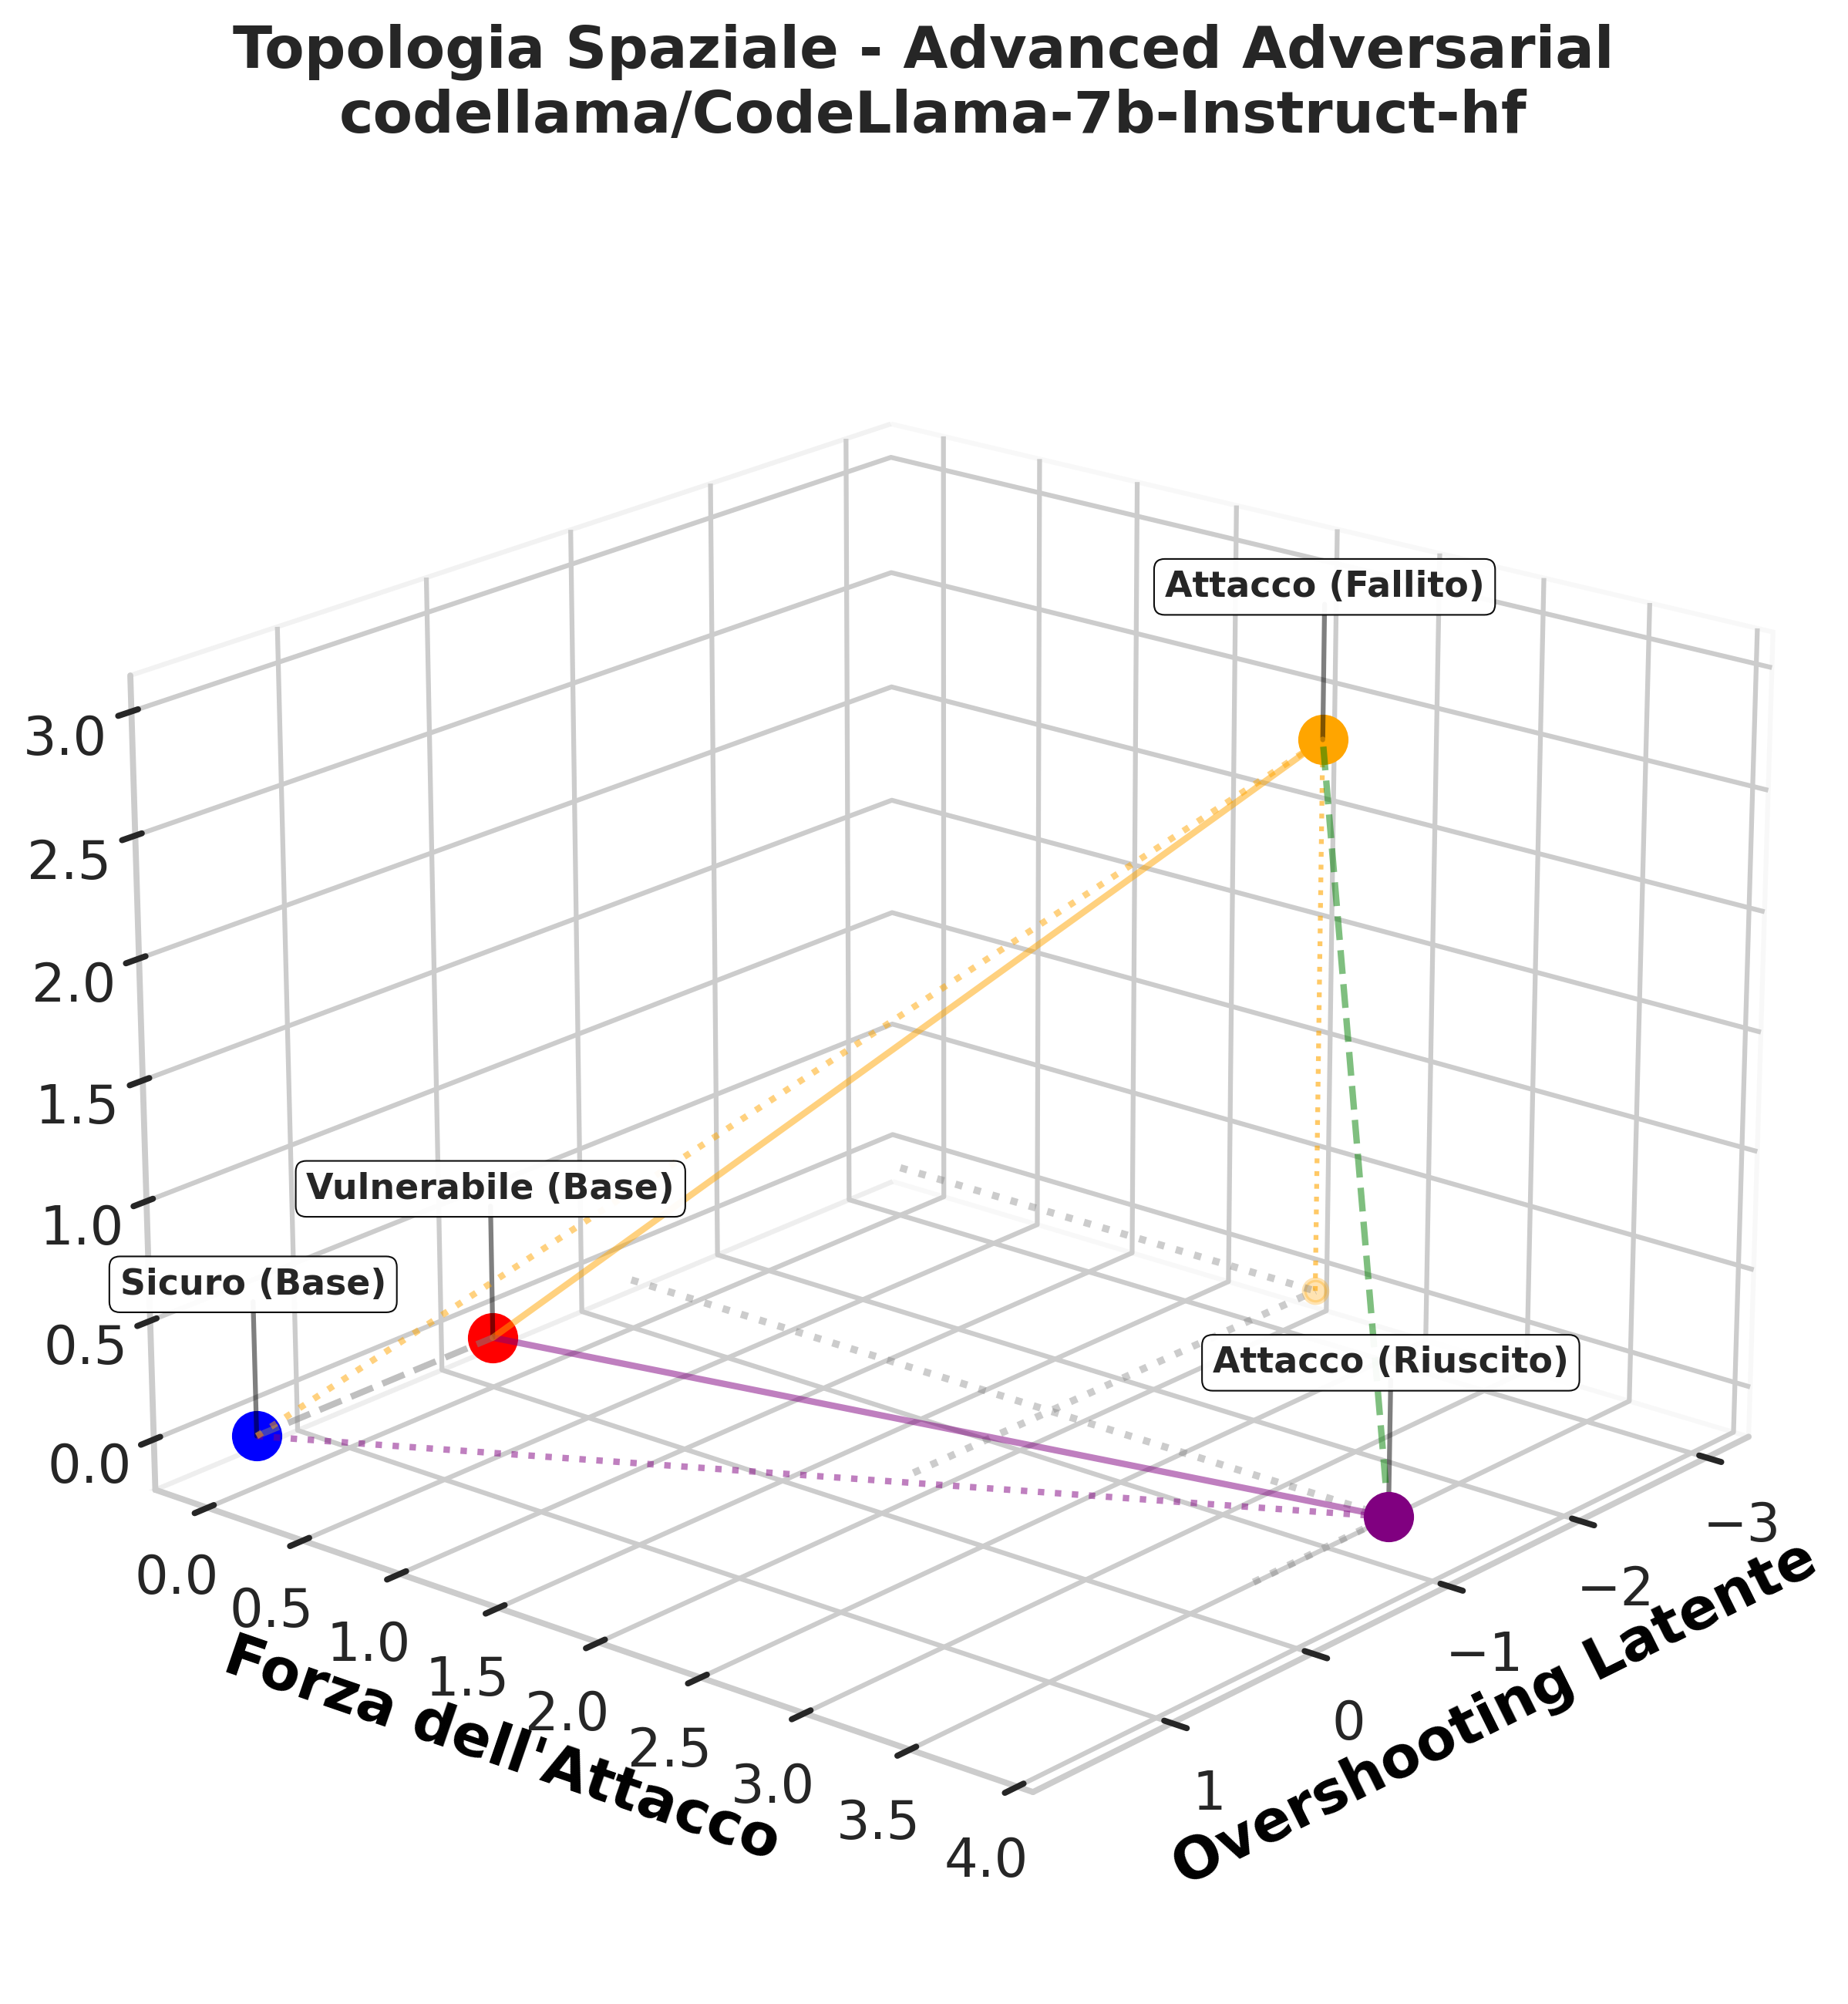
\includegraphics[width=\textwidth]{immagini/SWEEP L2/AA_Topologia3D_codellama_CodeLlama-7b-Instruct-hf_13.png}
        \caption{CodeLlama-7b-Instruct-hf}
       \end{subfigure}
\end{figure}


\begin{figure}[H]
    \centering
    \begin{subfigure}[b]{0.45\textwidth}
        \centering
        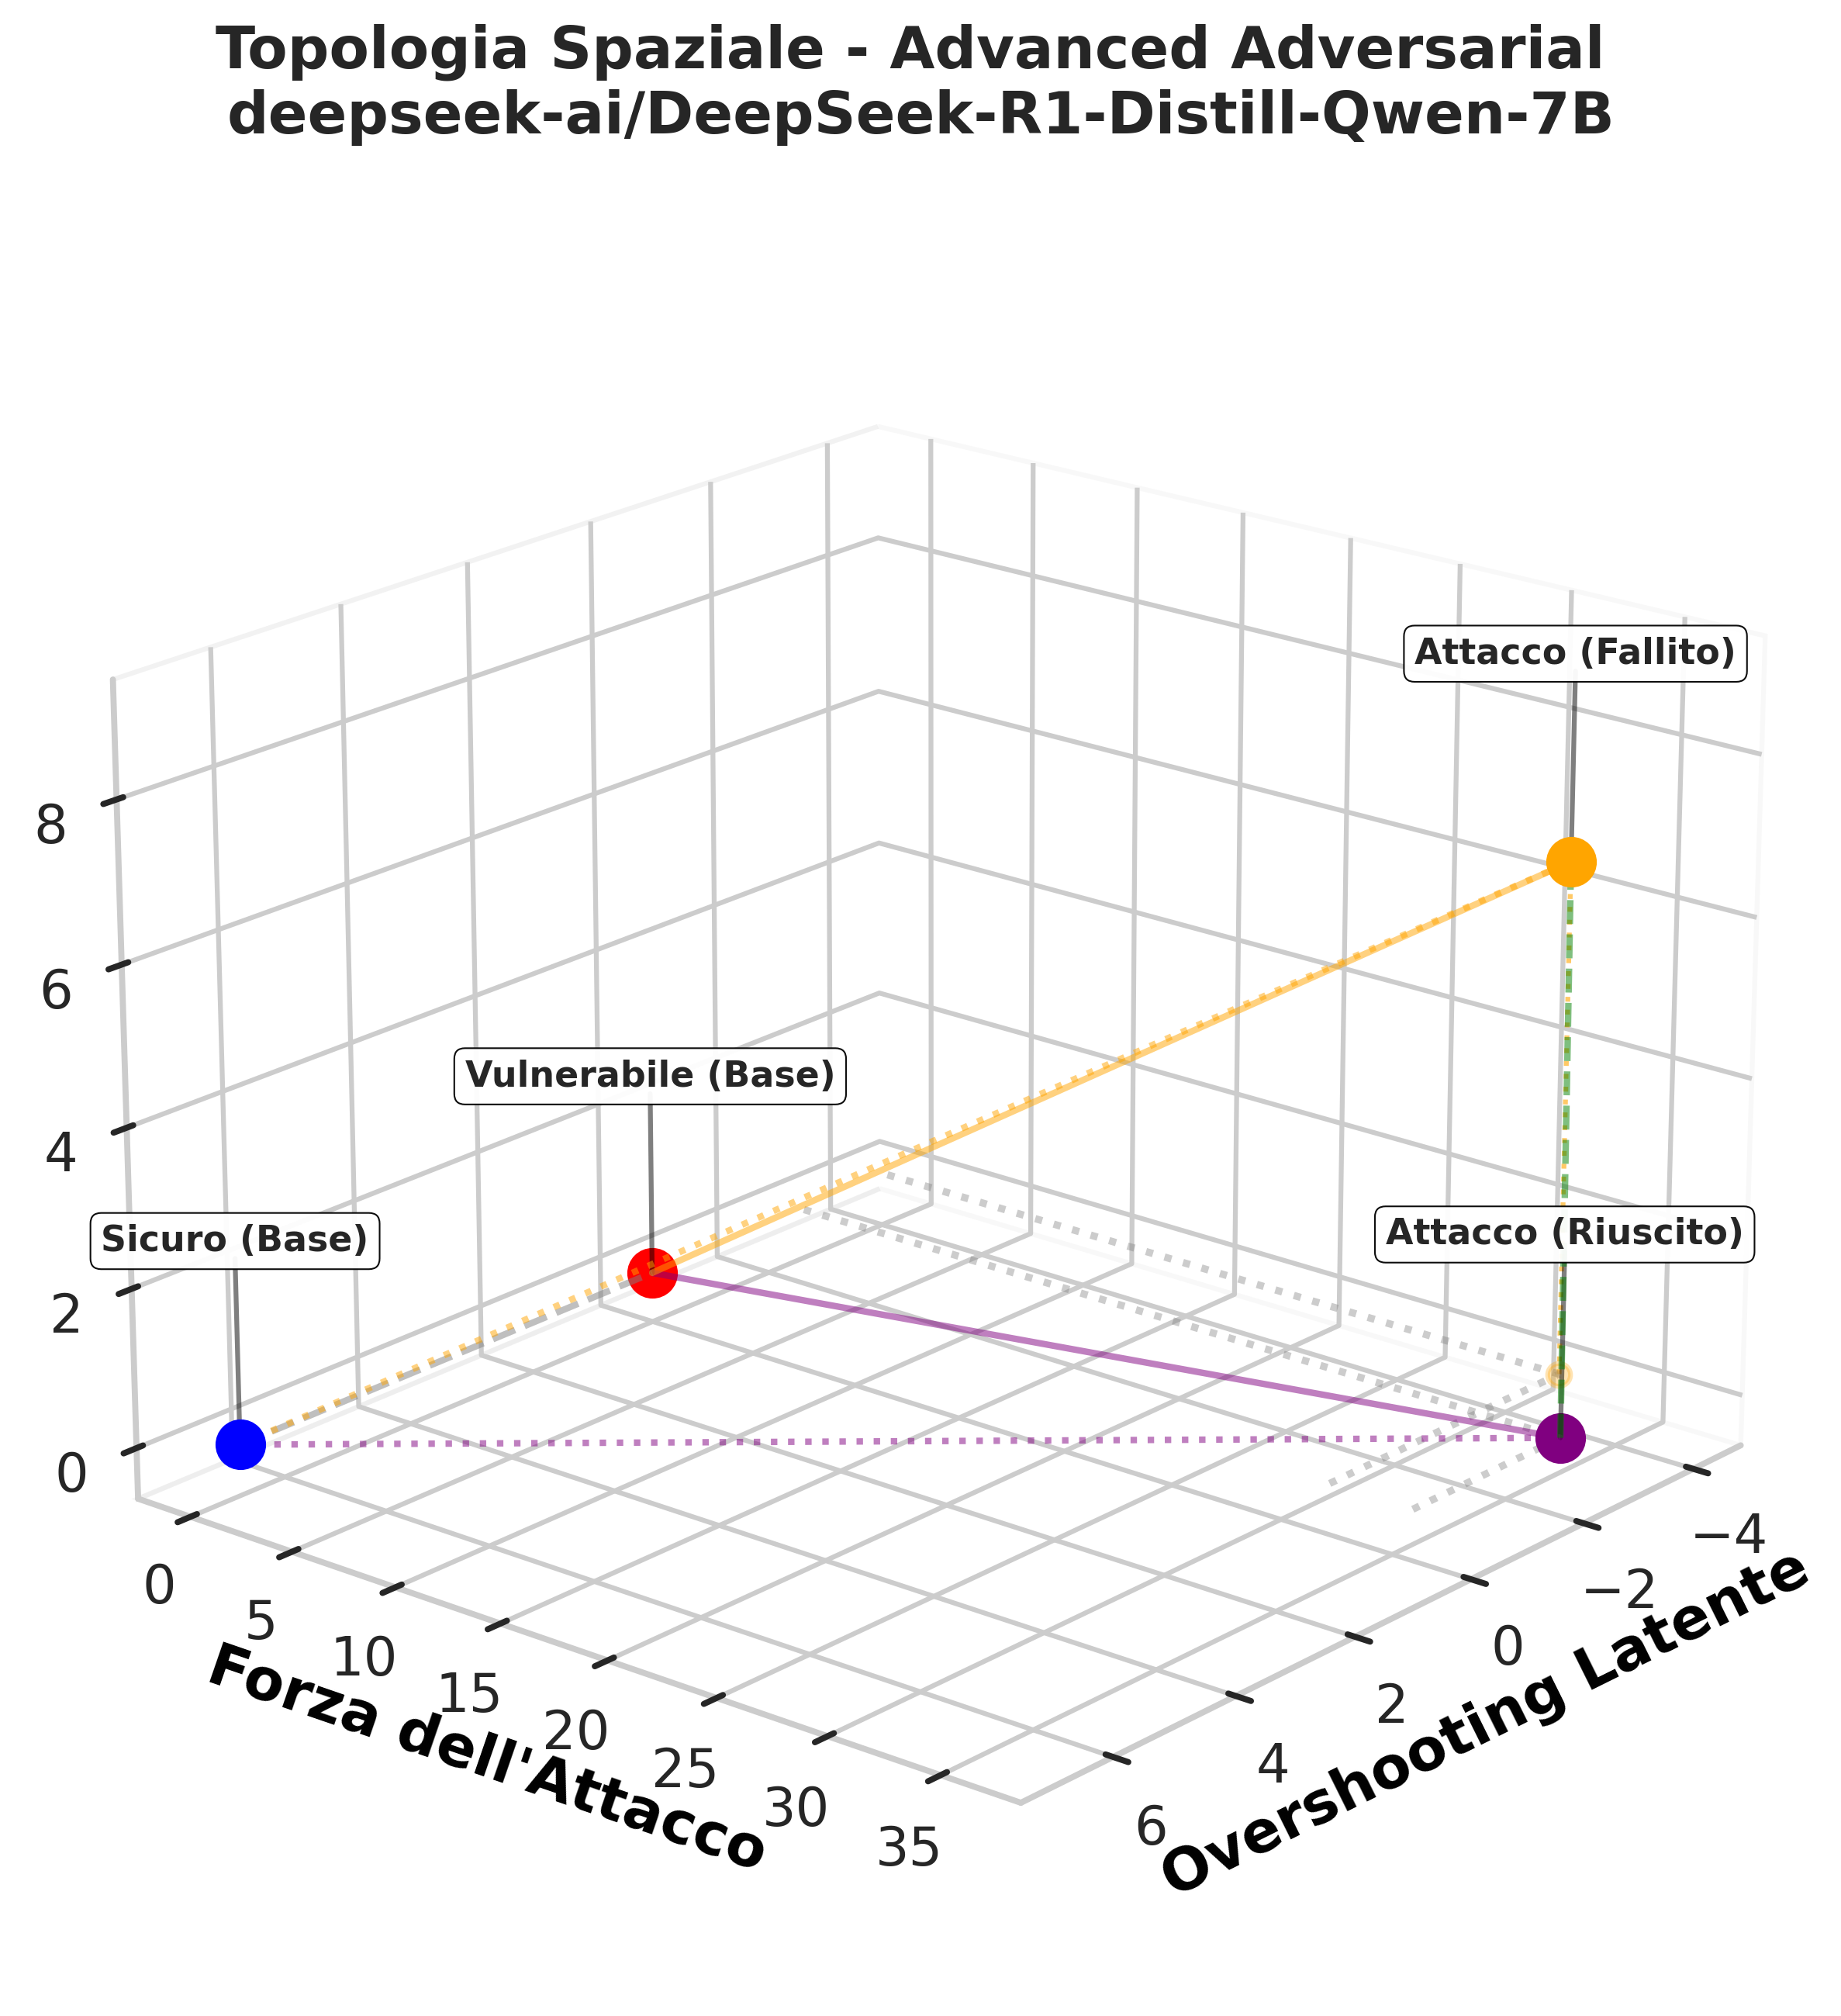
\includegraphics[width=\textwidth]{immagini/SWEEP L2/AA_Topologia3D_deepseek-ai_DeepSeek-R1-Distill-Qwen-7B_19.png} 
        \caption{DeepSeek-R1-Distill-Qwen-7B}
    \end{subfigure}
    \hfill 
    \begin{subfigure}[b]{0.45\textwidth}
        \centering
        
\includegraphics[width=\textwidth]{immagini/SWEEP L2/AA_Topologia3D_deepseek-ai_deepseek-coder-6.7b-instruct_16.png}
        \caption{deepseek-coder-6.7b-instruct}
    \end{subfigure}
\end{figure}

\section{Adversarial Perturbation}

\begin{figure}[H]
    \centering
    \begin{subfigure}[b]{0.45\textwidth}
        \centering
        
\includegraphics[width=\textwidth]{immagini/SWEEP L2/AP_Topologia3D_Qwen_Qwen2.5-7B-Instruct_18.png} 
        \caption{Qwen2.5-7B-Instruct}
    \end{subfigure}
    \hfill 
    \begin{subfigure}[b]{0.45\textwidth}
        \centering
        
\includegraphics[width=\textwidth]{immagini/SWEEP L2/AP_Topologia3D_Qwen_Qwen2.5-Coder-7B-Instruct_18.png}
        \caption{Qwen2.5-Coder-7B-Instruct}
    \end{subfigure}
\end{figure}

\begin{figure}[H]
    \centering
    \begin{subfigure}[b]{0.45\textwidth}
        \centering
        
\includegraphics[width=\textwidth]{immagini/SWEEP L2/AP_Topologia3D_meta-llama_Llama-3.1-8B-Instruct_15.png} 
        \caption{Llama-3.1-8B-Instruct}
    \end{subfigure}
    \hfill 
    \begin{subfigure}[b]{0.45\textwidth}
        \centering
        
\includegraphics[width=\textwidth]{immagini/SWEEP L2/AP_Topologia3D_codellama_CodeLlama-7b-Instruct-hf_13.png}
        \caption{CodeLlama-7b-Instruct-hf}
    \end{subfigure}
\end{figure}

\begin{figure}[H]
    \centering
    \begin{subfigure}[b]{0.45\textwidth}
        \centering
        
\includegraphics[width=\textwidth]{immagini/SWEEP L2/AP_Topologia3D_Qwen_Qwen2.5-7B-Instruct_18.png} 
        \caption{DeepSeek-R1-Distill-Qwen-7B}
    \end{subfigure}
    \hfill 
    \begin{subfigure}[b]{0.45\textwidth}
        \centering
        
\includegraphics[width=\textwidth]{immagini/SWEEP L2/AP_Topologia3D_deepseek-ai_deepseek-coder-6.7b-instruct_16.png}
        \caption{deepseek-coder-6.7b-instruct}
    \end{subfigure}
\end{figure}

\section{Prompt Injection}

\begin{figure}[H]
    \centering
    \begin{subfigure}[b]{0.45\textwidth}
        \centering
        
\includegraphics[width=\textwidth]{immagini/SWEEP L2/PI_Topologia3D_Qwen_Qwen2.5-7B-Instruct_18.png} 
        \caption{Qwen2.5-7B-Instruct}
    \end{subfigure}
    \hfill 
    \begin{subfigure}[b]{0.45\textwidth}
        \centering
        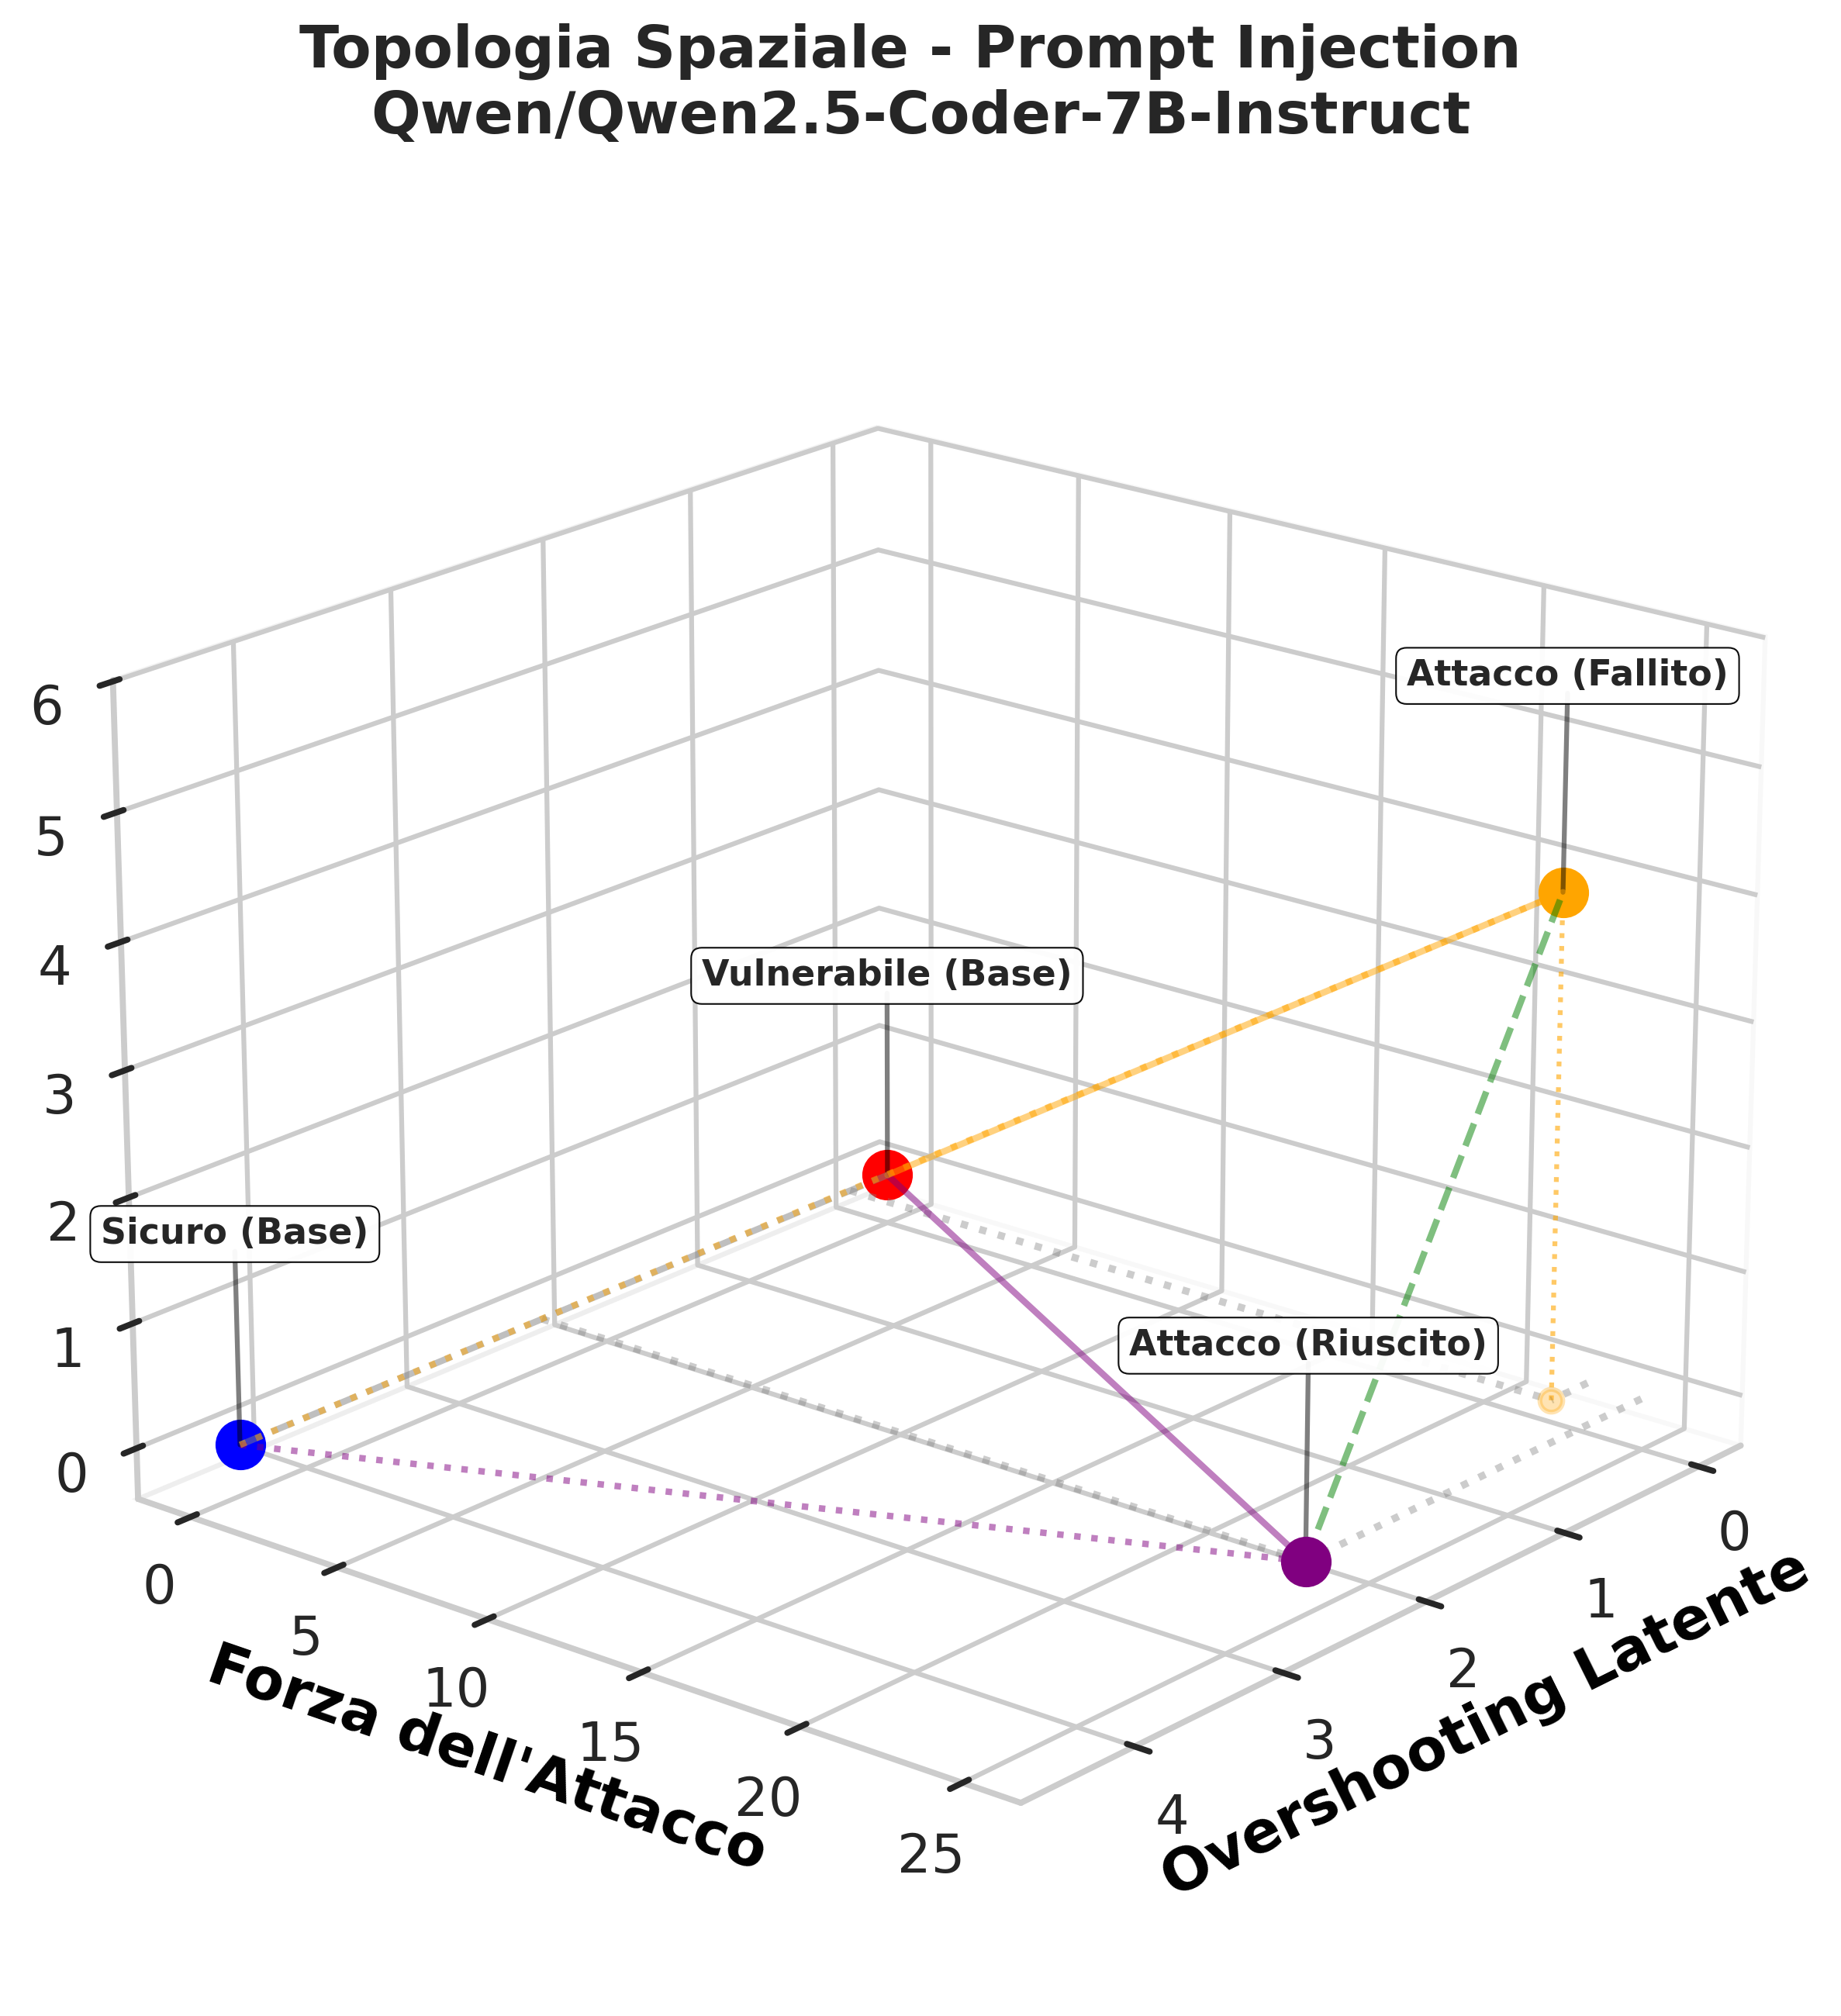
\includegraphics[width=\textwidth]{immagini/SWEEP L2/PI_Topologia3D_Qwen_Qwen2.5-Coder-7B-Instruct_18.png}
        \caption{Qwen2.5-Coder-7B-Instruct}
    \end{subfigure}
\end{figure}

\begin{figure}[H]
    \centering
    \begin{subfigure}[b]{0.45\textwidth}
        \centering
        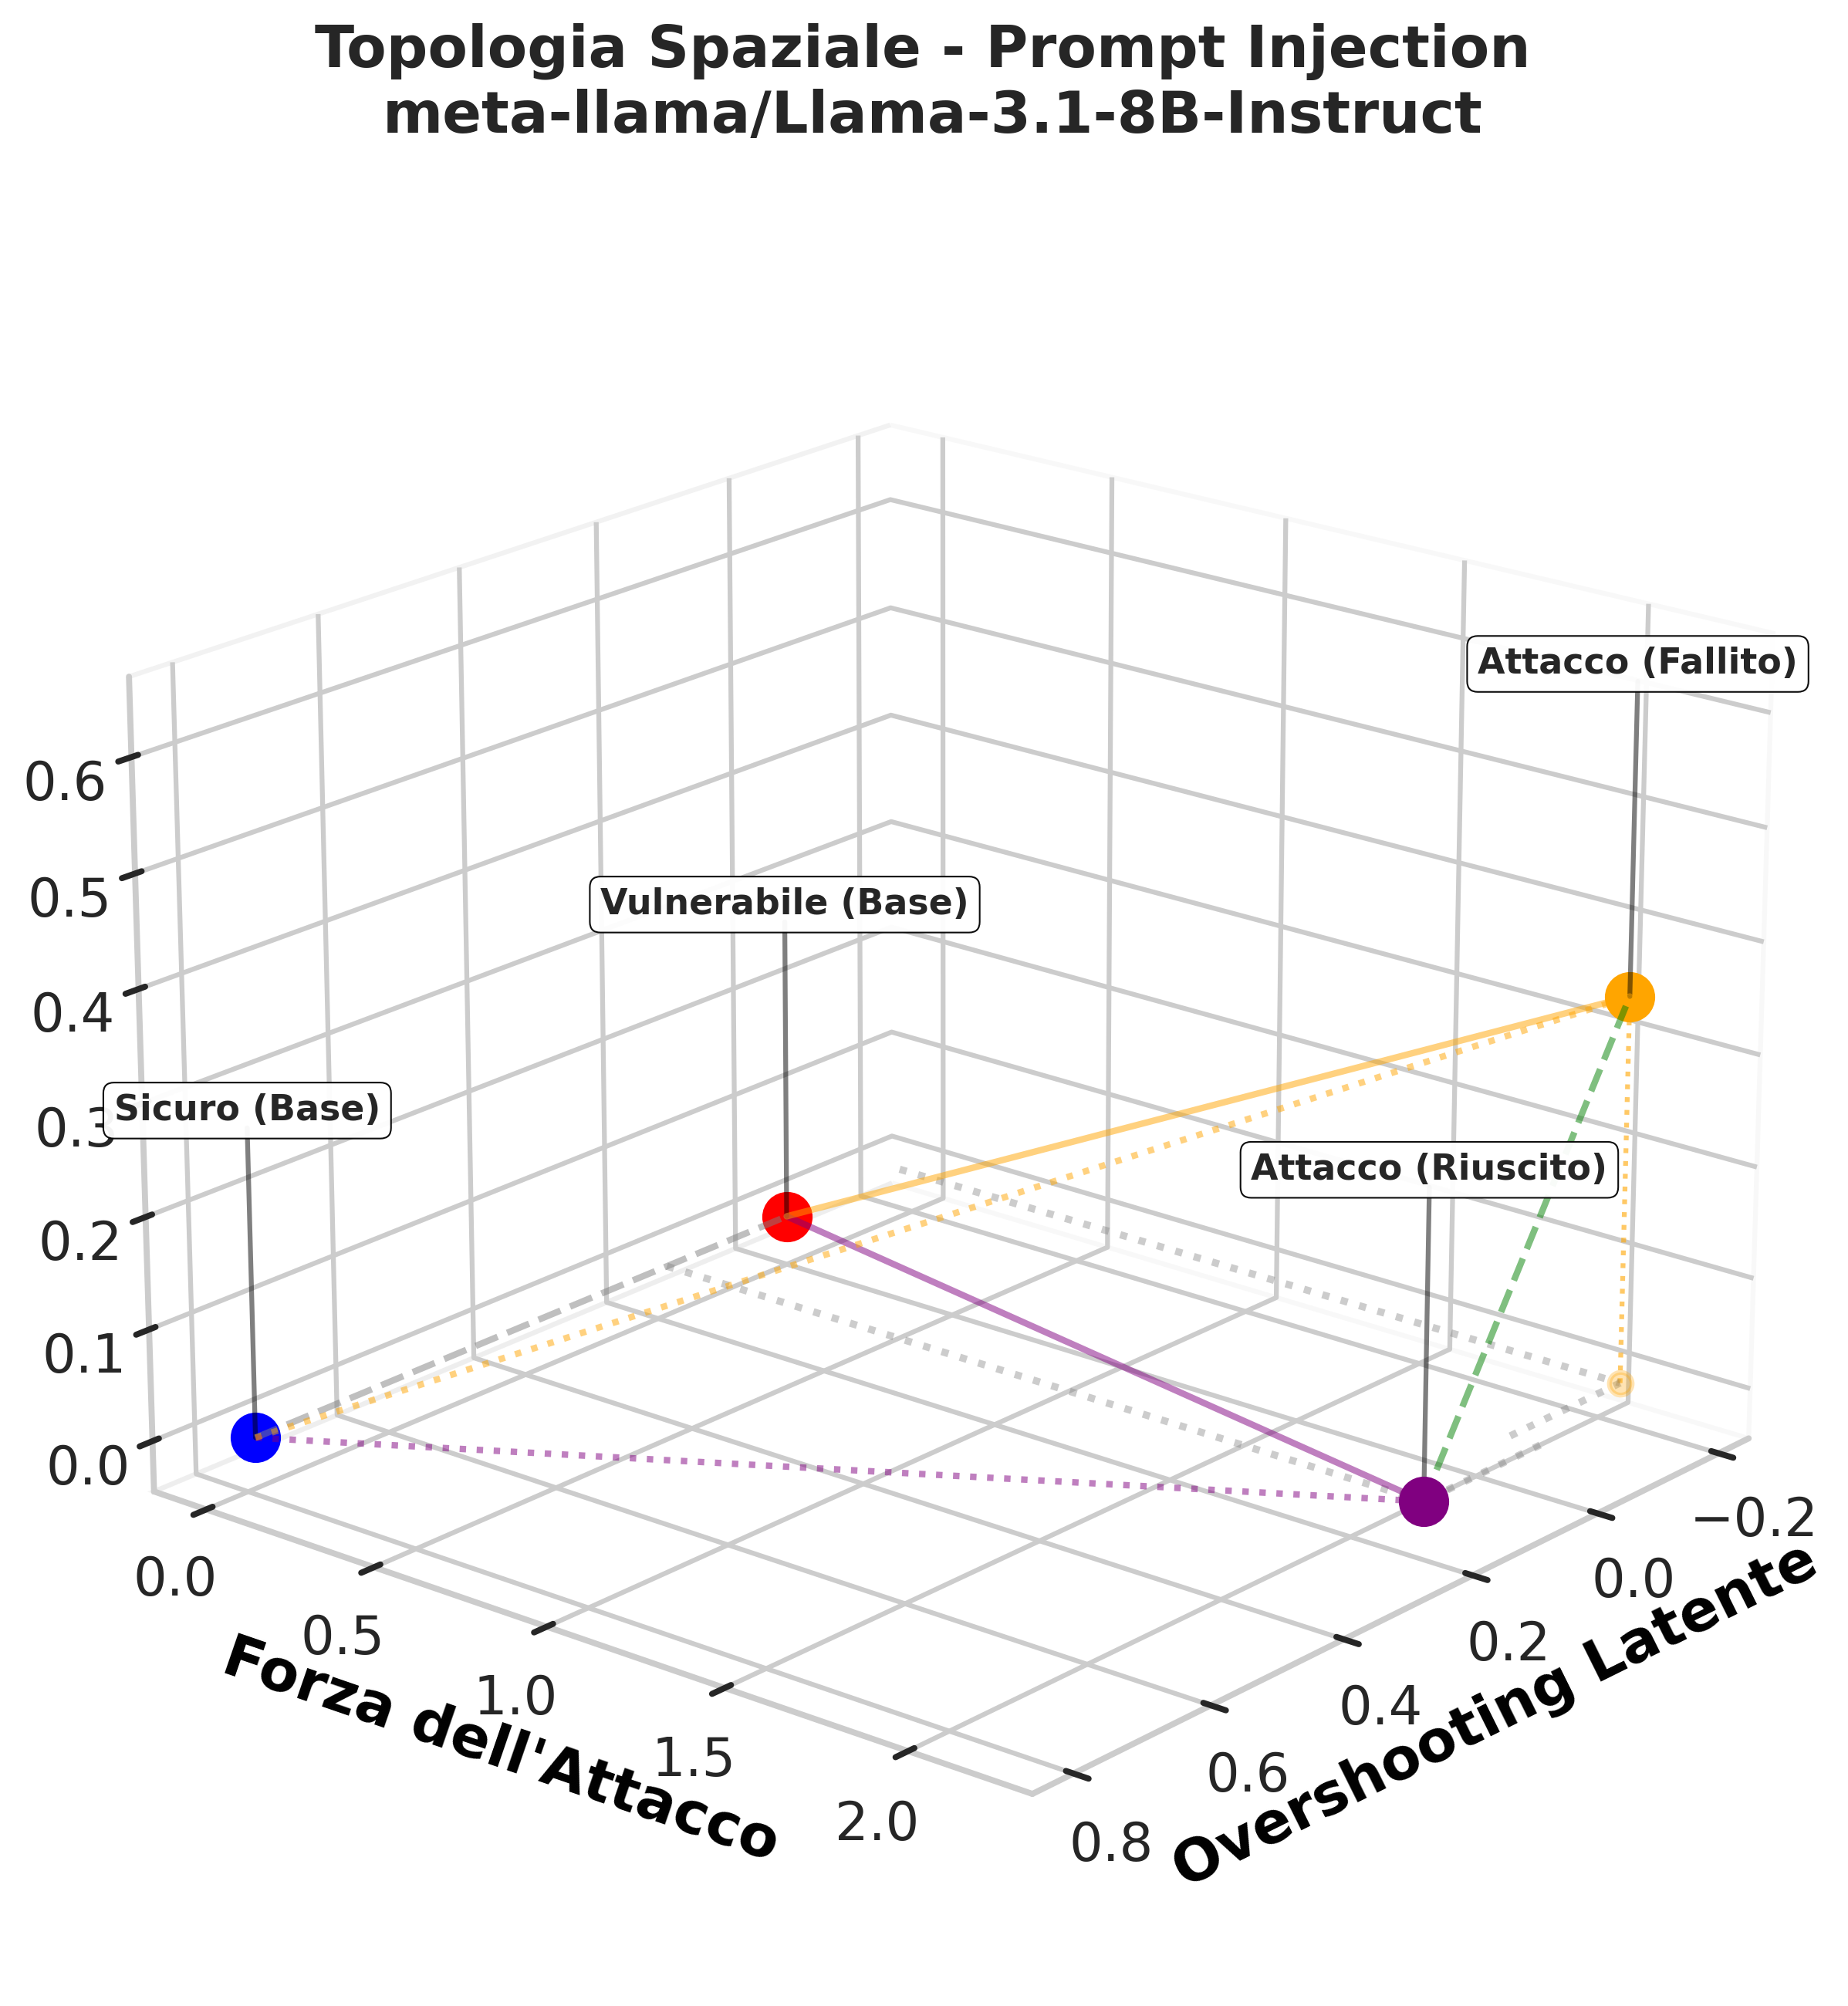
\includegraphics[width=\textwidth]{immagini/SWEEP L2/PI_Topologia3D_meta-llama_Llama-3.1-8B-Instruct_15.png} 
        \caption{Llama-3.1-8B-Instruct}
    \end{subfigure}
    \hfill 
    \begin{subfigure}[b]{0.45\textwidth}
        \centering
        
\includegraphics[width=\textwidth]{immagini/SWEEP L2/PI_Topologia3D_codellama_CodeLlama-7b-Instruct-hf_13.png}
        \caption{CodeLlama-7b-Instruct-hf}
    \end{subfigure}
\end{figure}

\begin{figure}[H]
    \centering
    \begin{subfigure}[b]{0.45\textwidth}
        \centering
        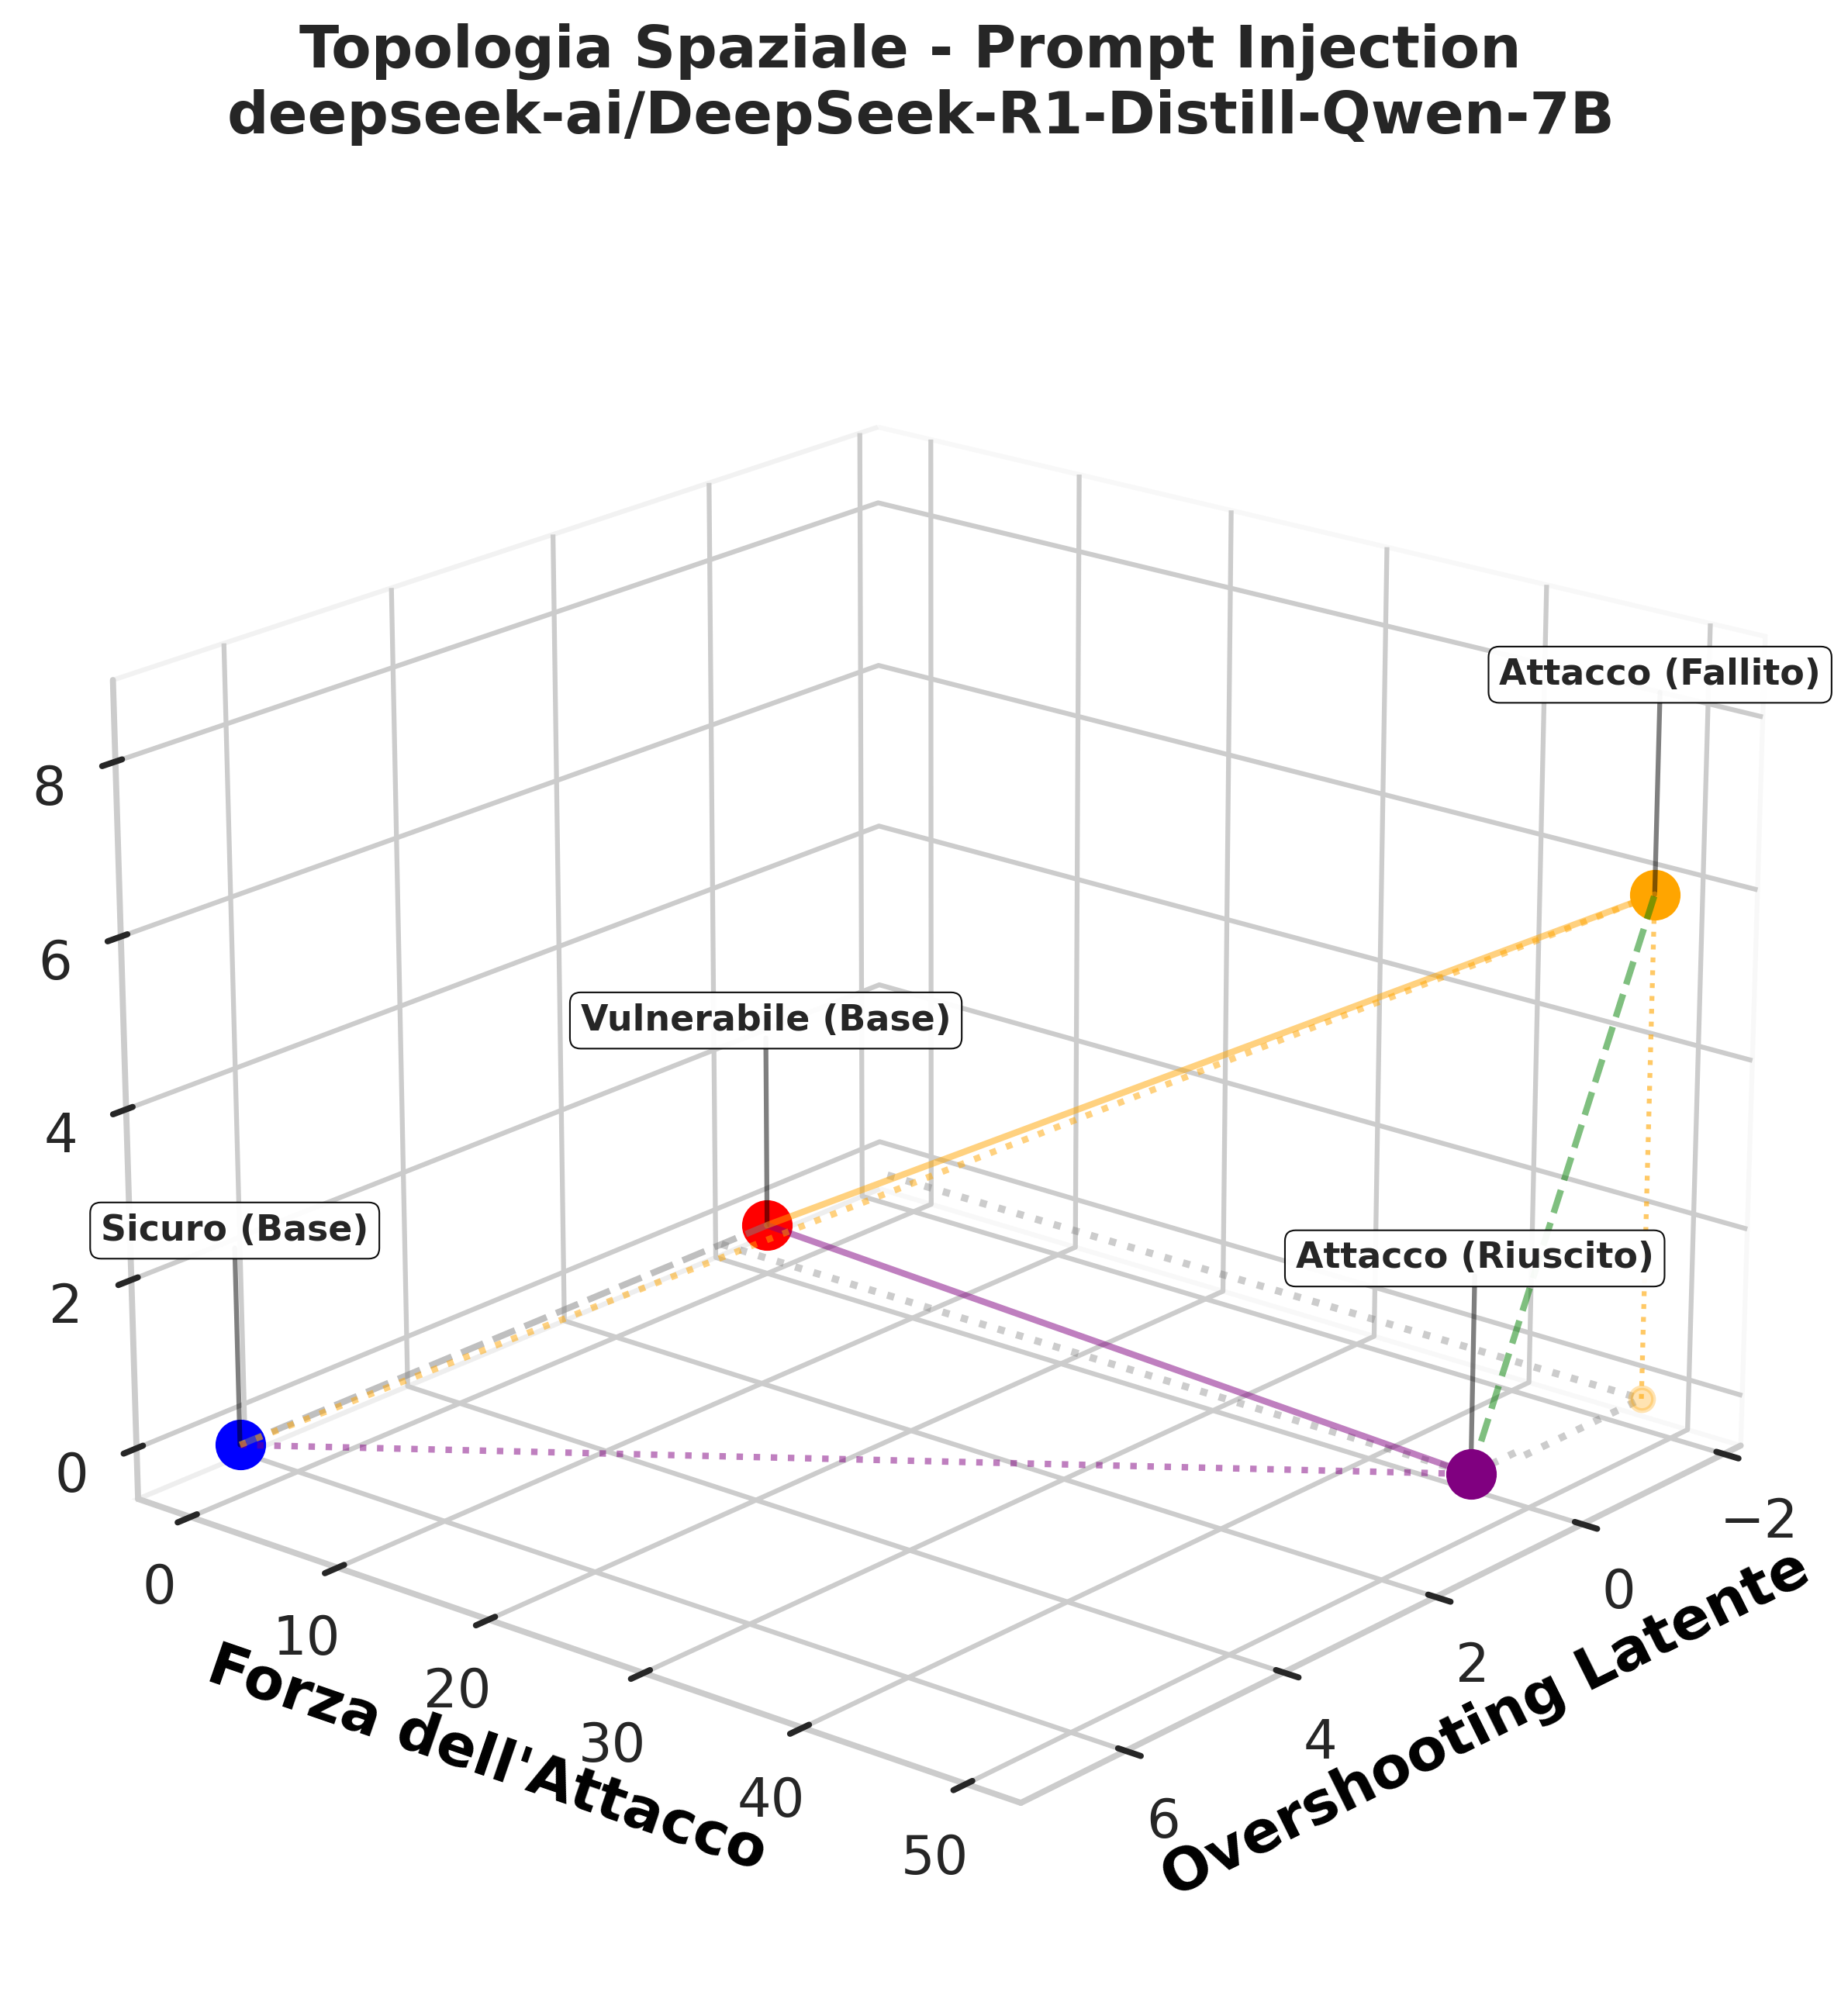
\includegraphics[width=\textwidth]{immagini/SWEEP L2/PI_Topologia3D_deepseek-ai_DeepSeek-R1-Distill-Qwen-7B_19.png} 
        \caption{DeepSeek-R1-Distill-Qwen-7B}
    \end{subfigure}
    \hfill 
    \begin{subfigure}[b]{0.45\textwidth}
        \centering
        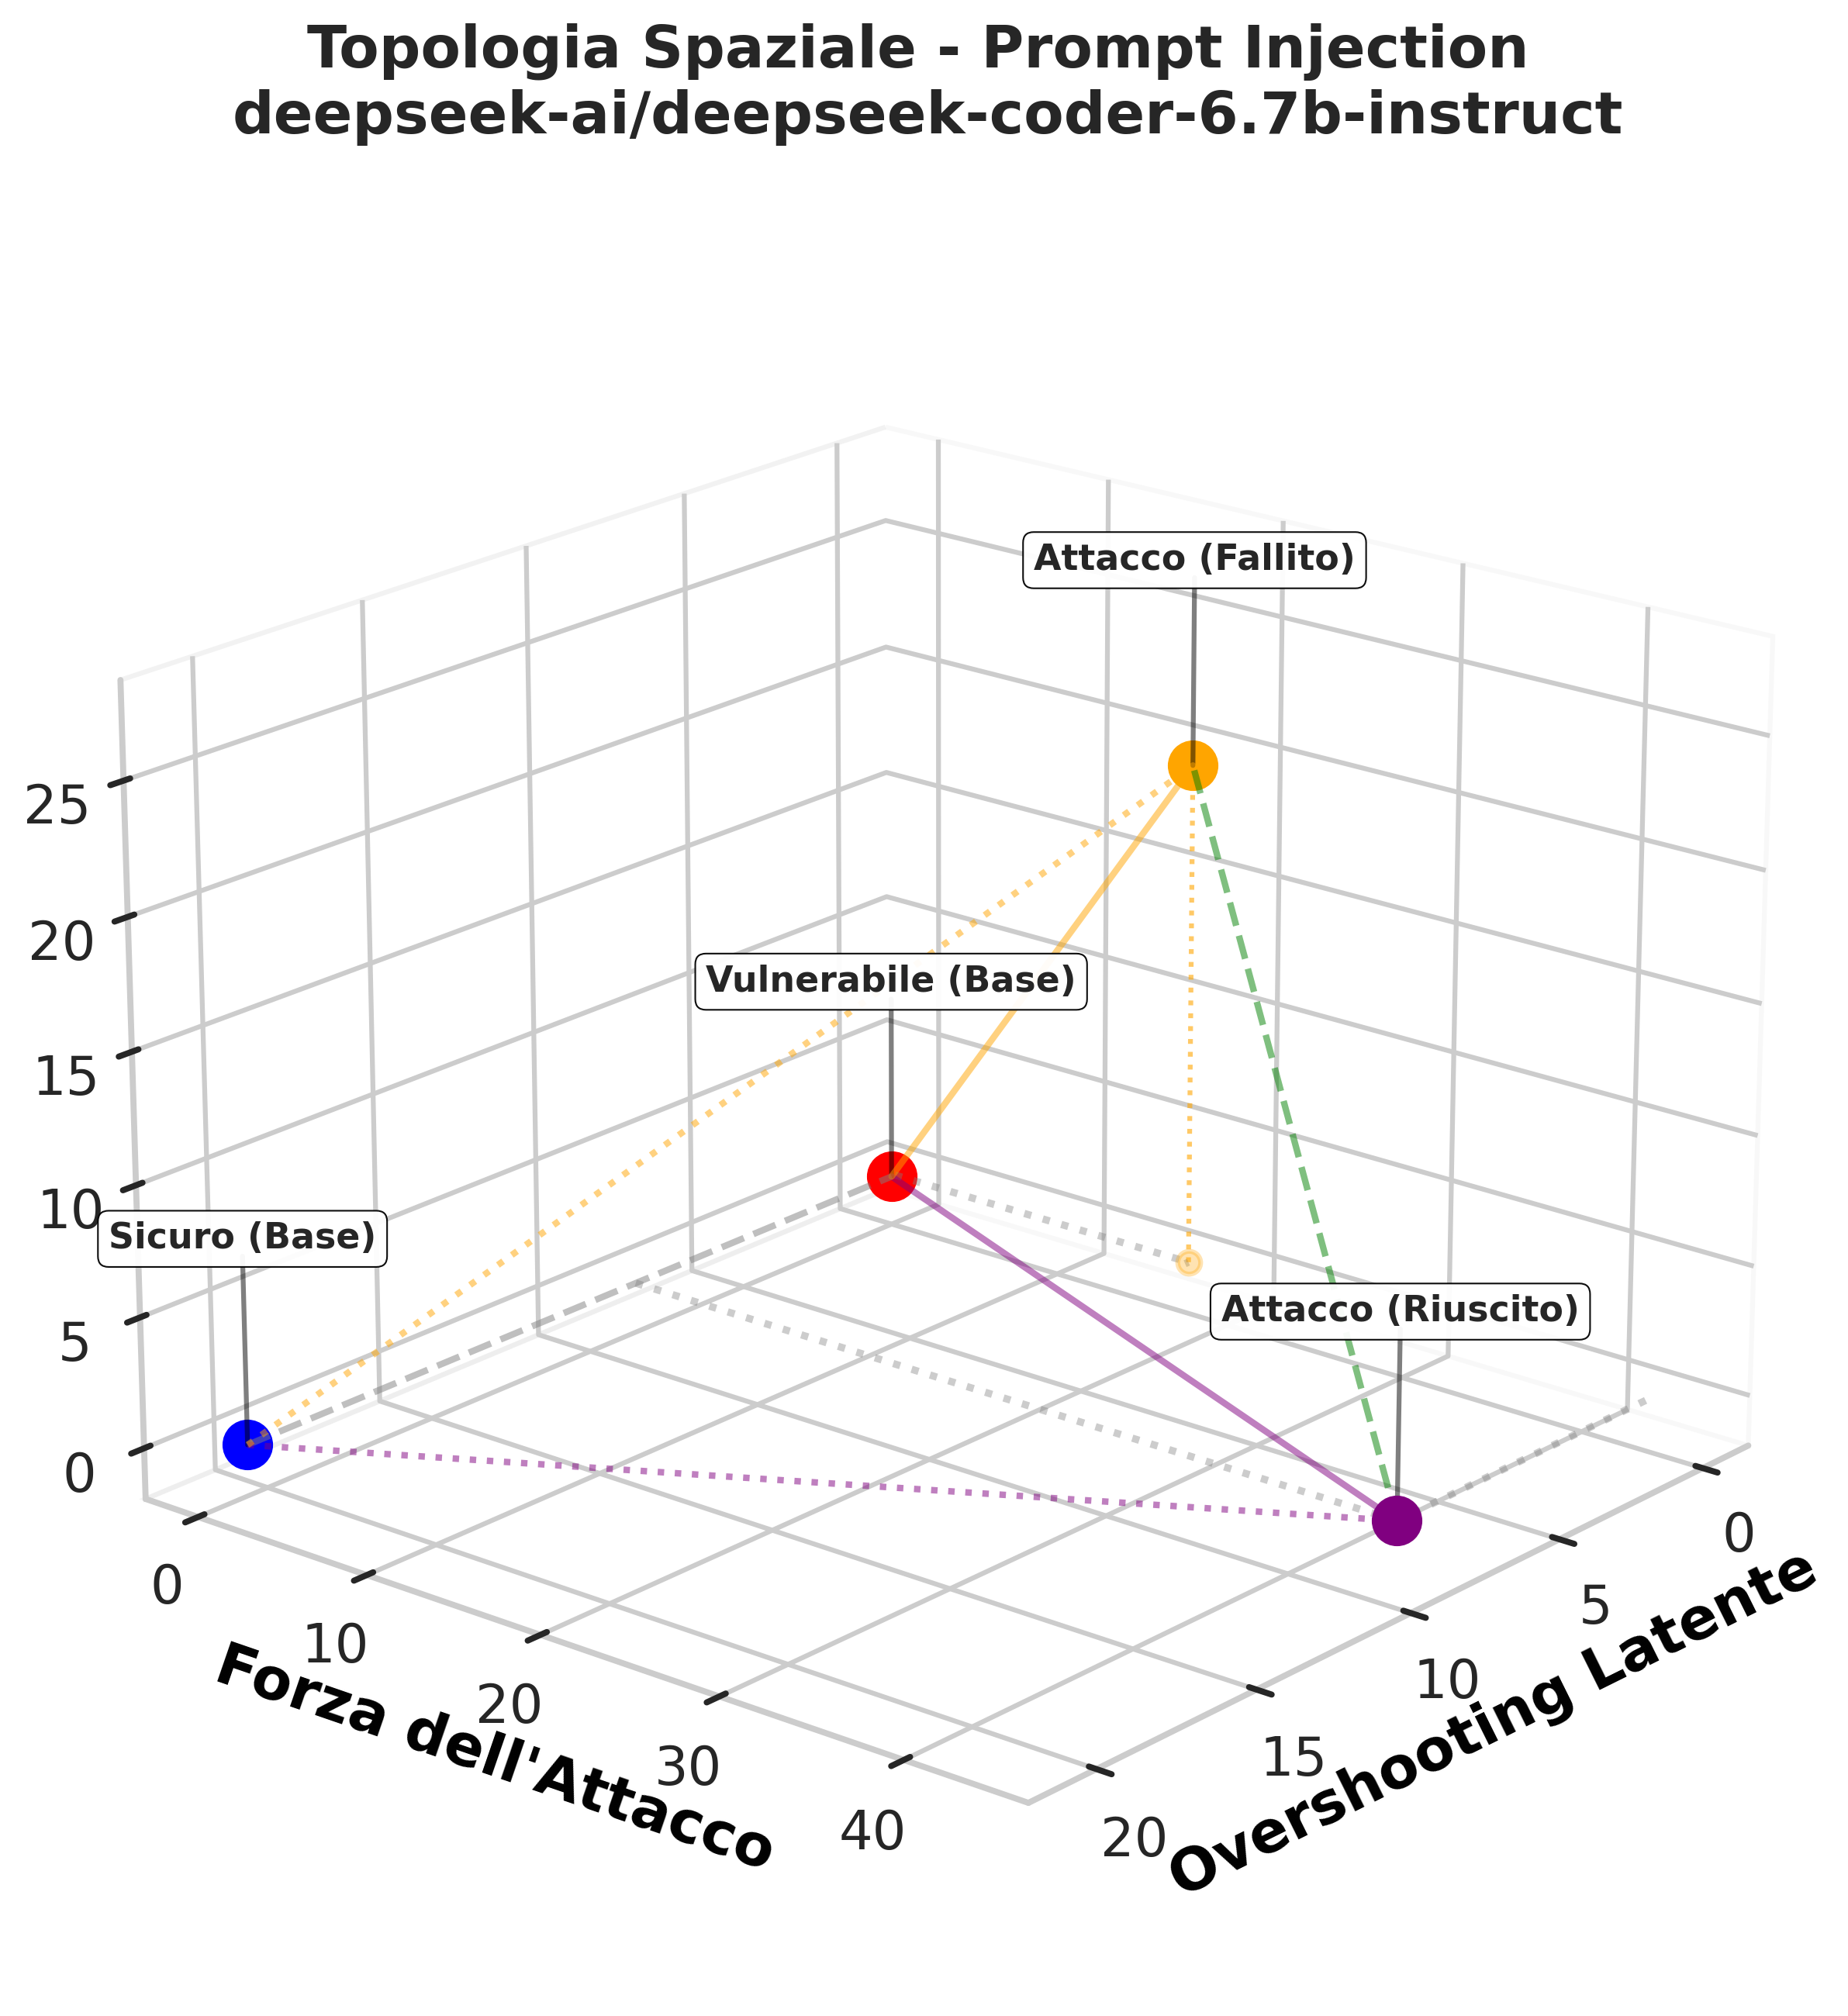
\includegraphics[width=\textwidth]{immagini/SWEEP L2/PI_Topologia3D_deepseek-ai_deepseek-coder-6.7b-instruct_16.png}
        \caption{deepseek-coder-6.7b-instruct}
    \end{subfigure}
\end{figure}

\section{Activation Steering}

\begin{figure}[H]
    \centering
    \begin{subfigure}[b]{0.45\textwidth}
        \centering
        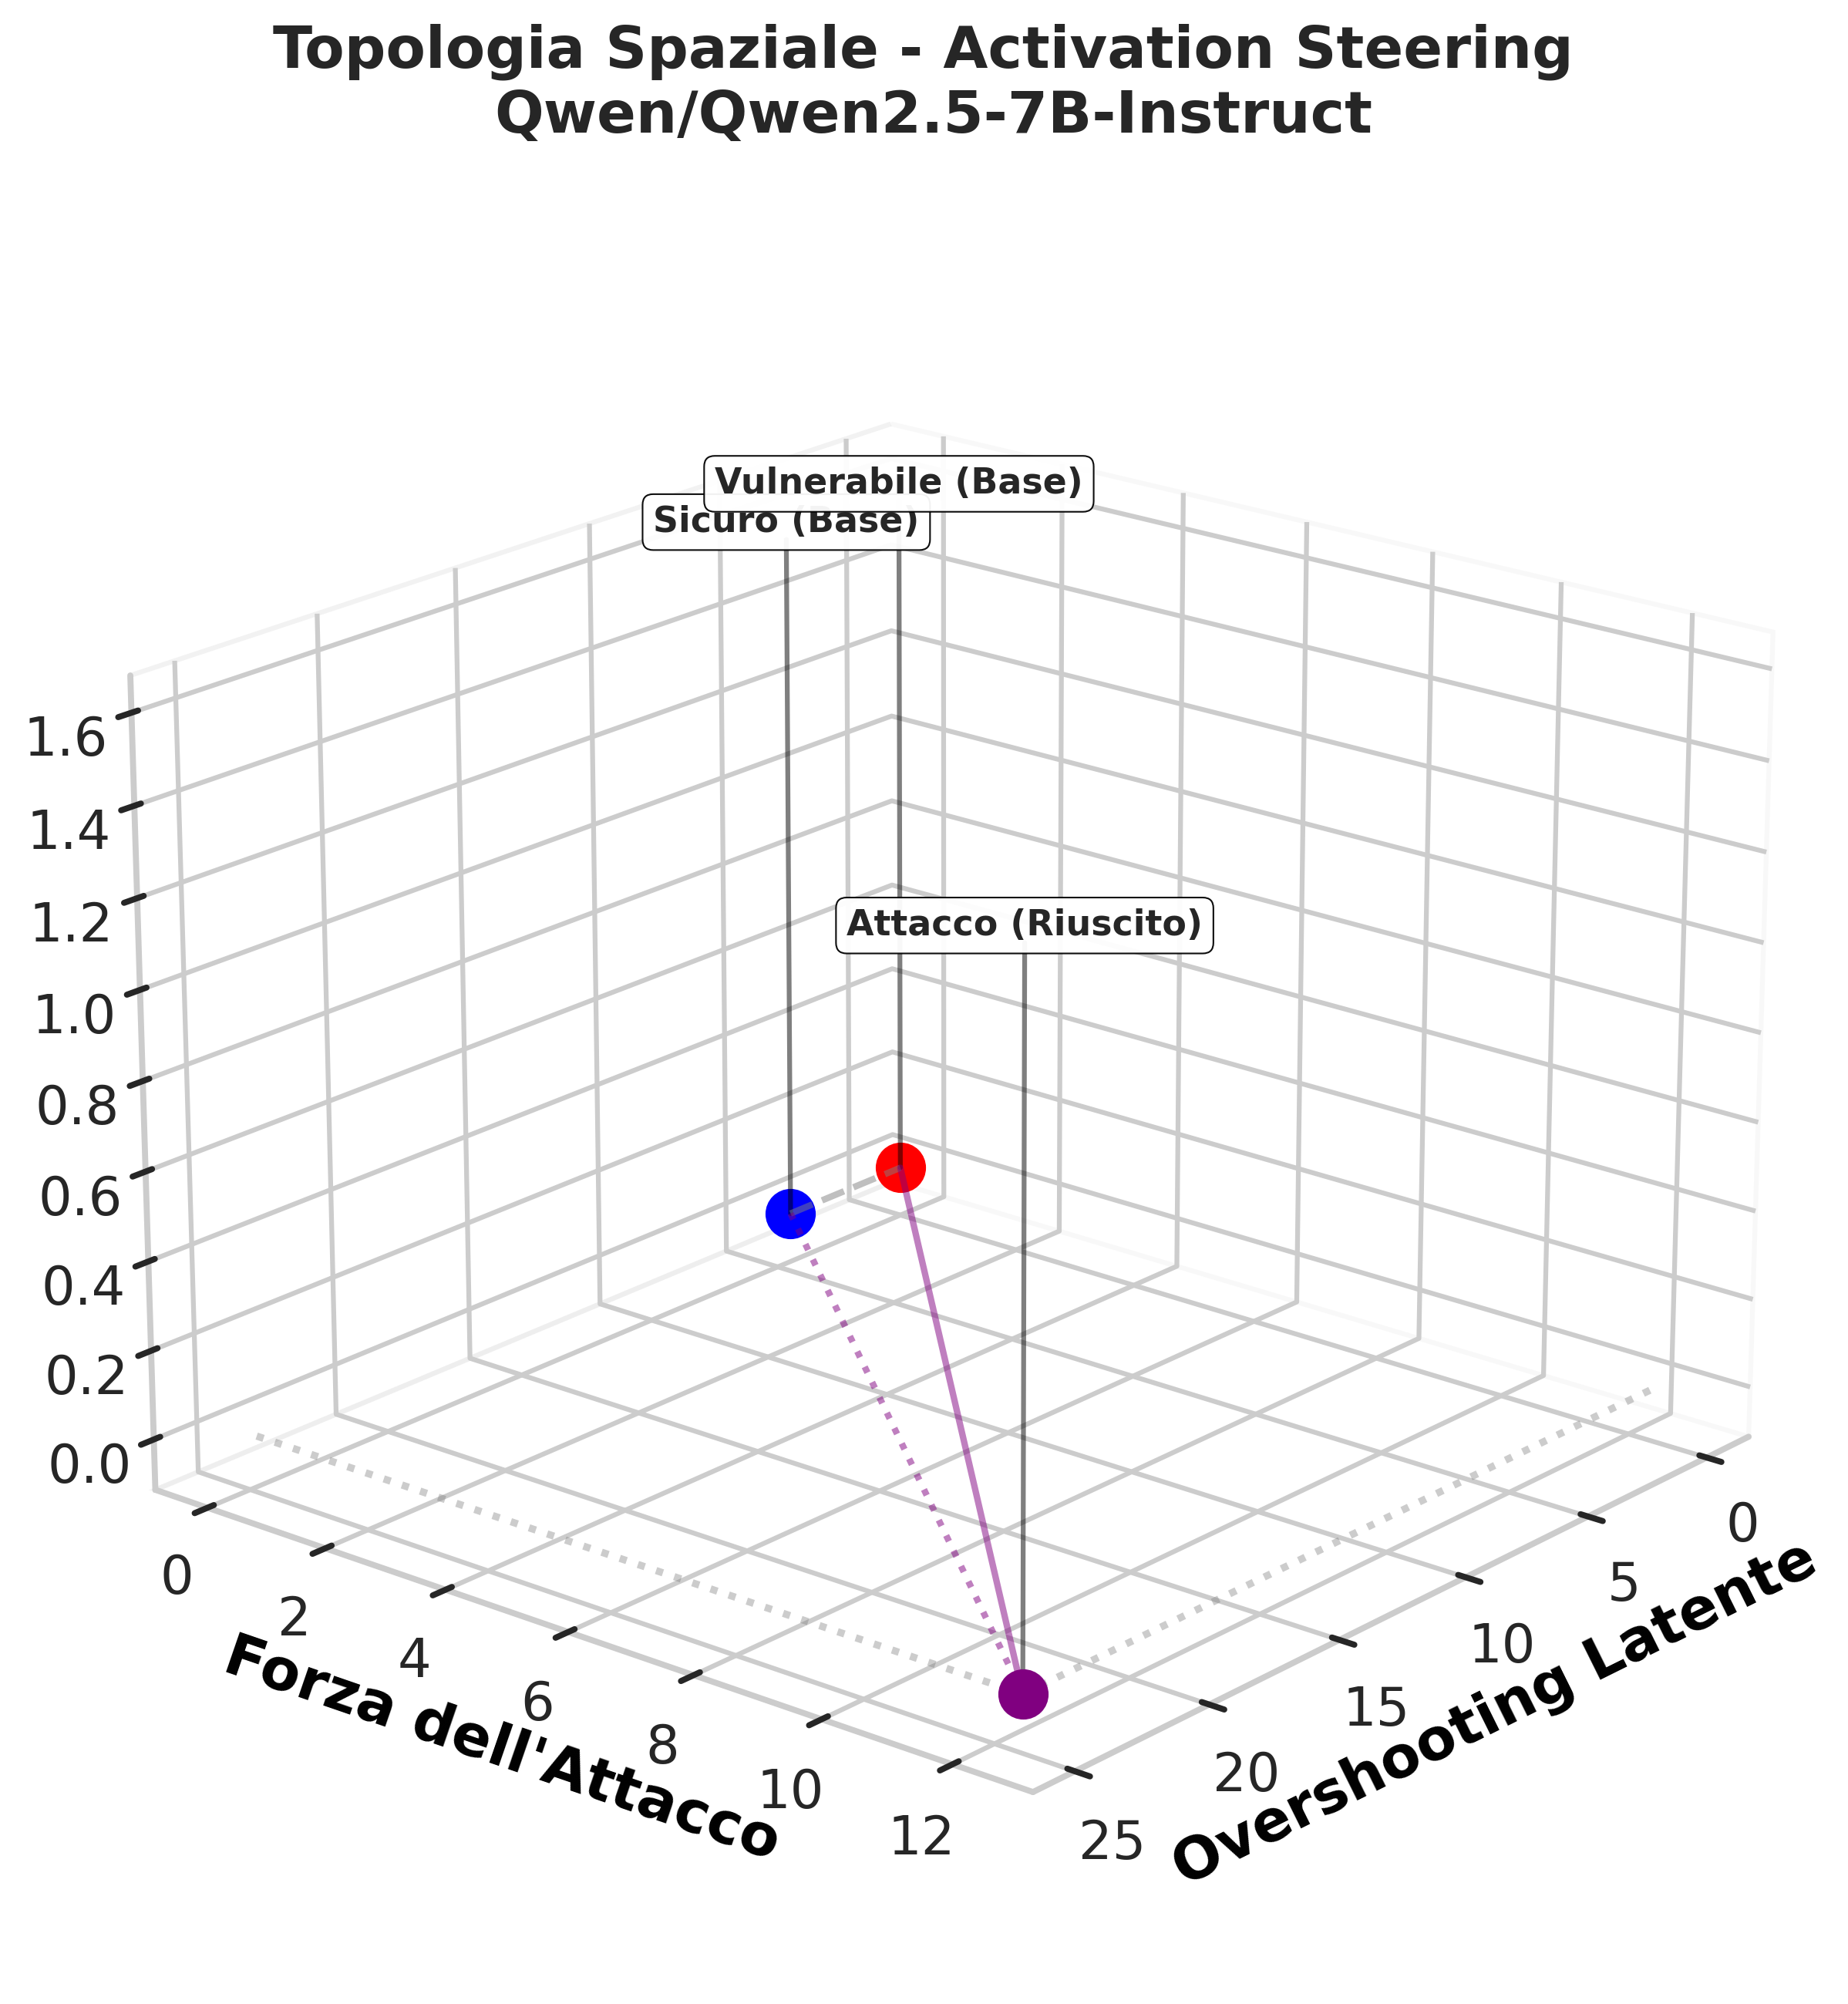
\includegraphics[width=\textwidth]{immagini/SWEEP L2/Steering_Topologia3D_Qwen_Qwen2.5-7B-Instruct_19.png} 
        \caption{Qwen2.5-7B-Instruct}
    \end{subfigure}
    \hfill 
    \begin{subfigure}[b]{0.45\textwidth}
        \centering
        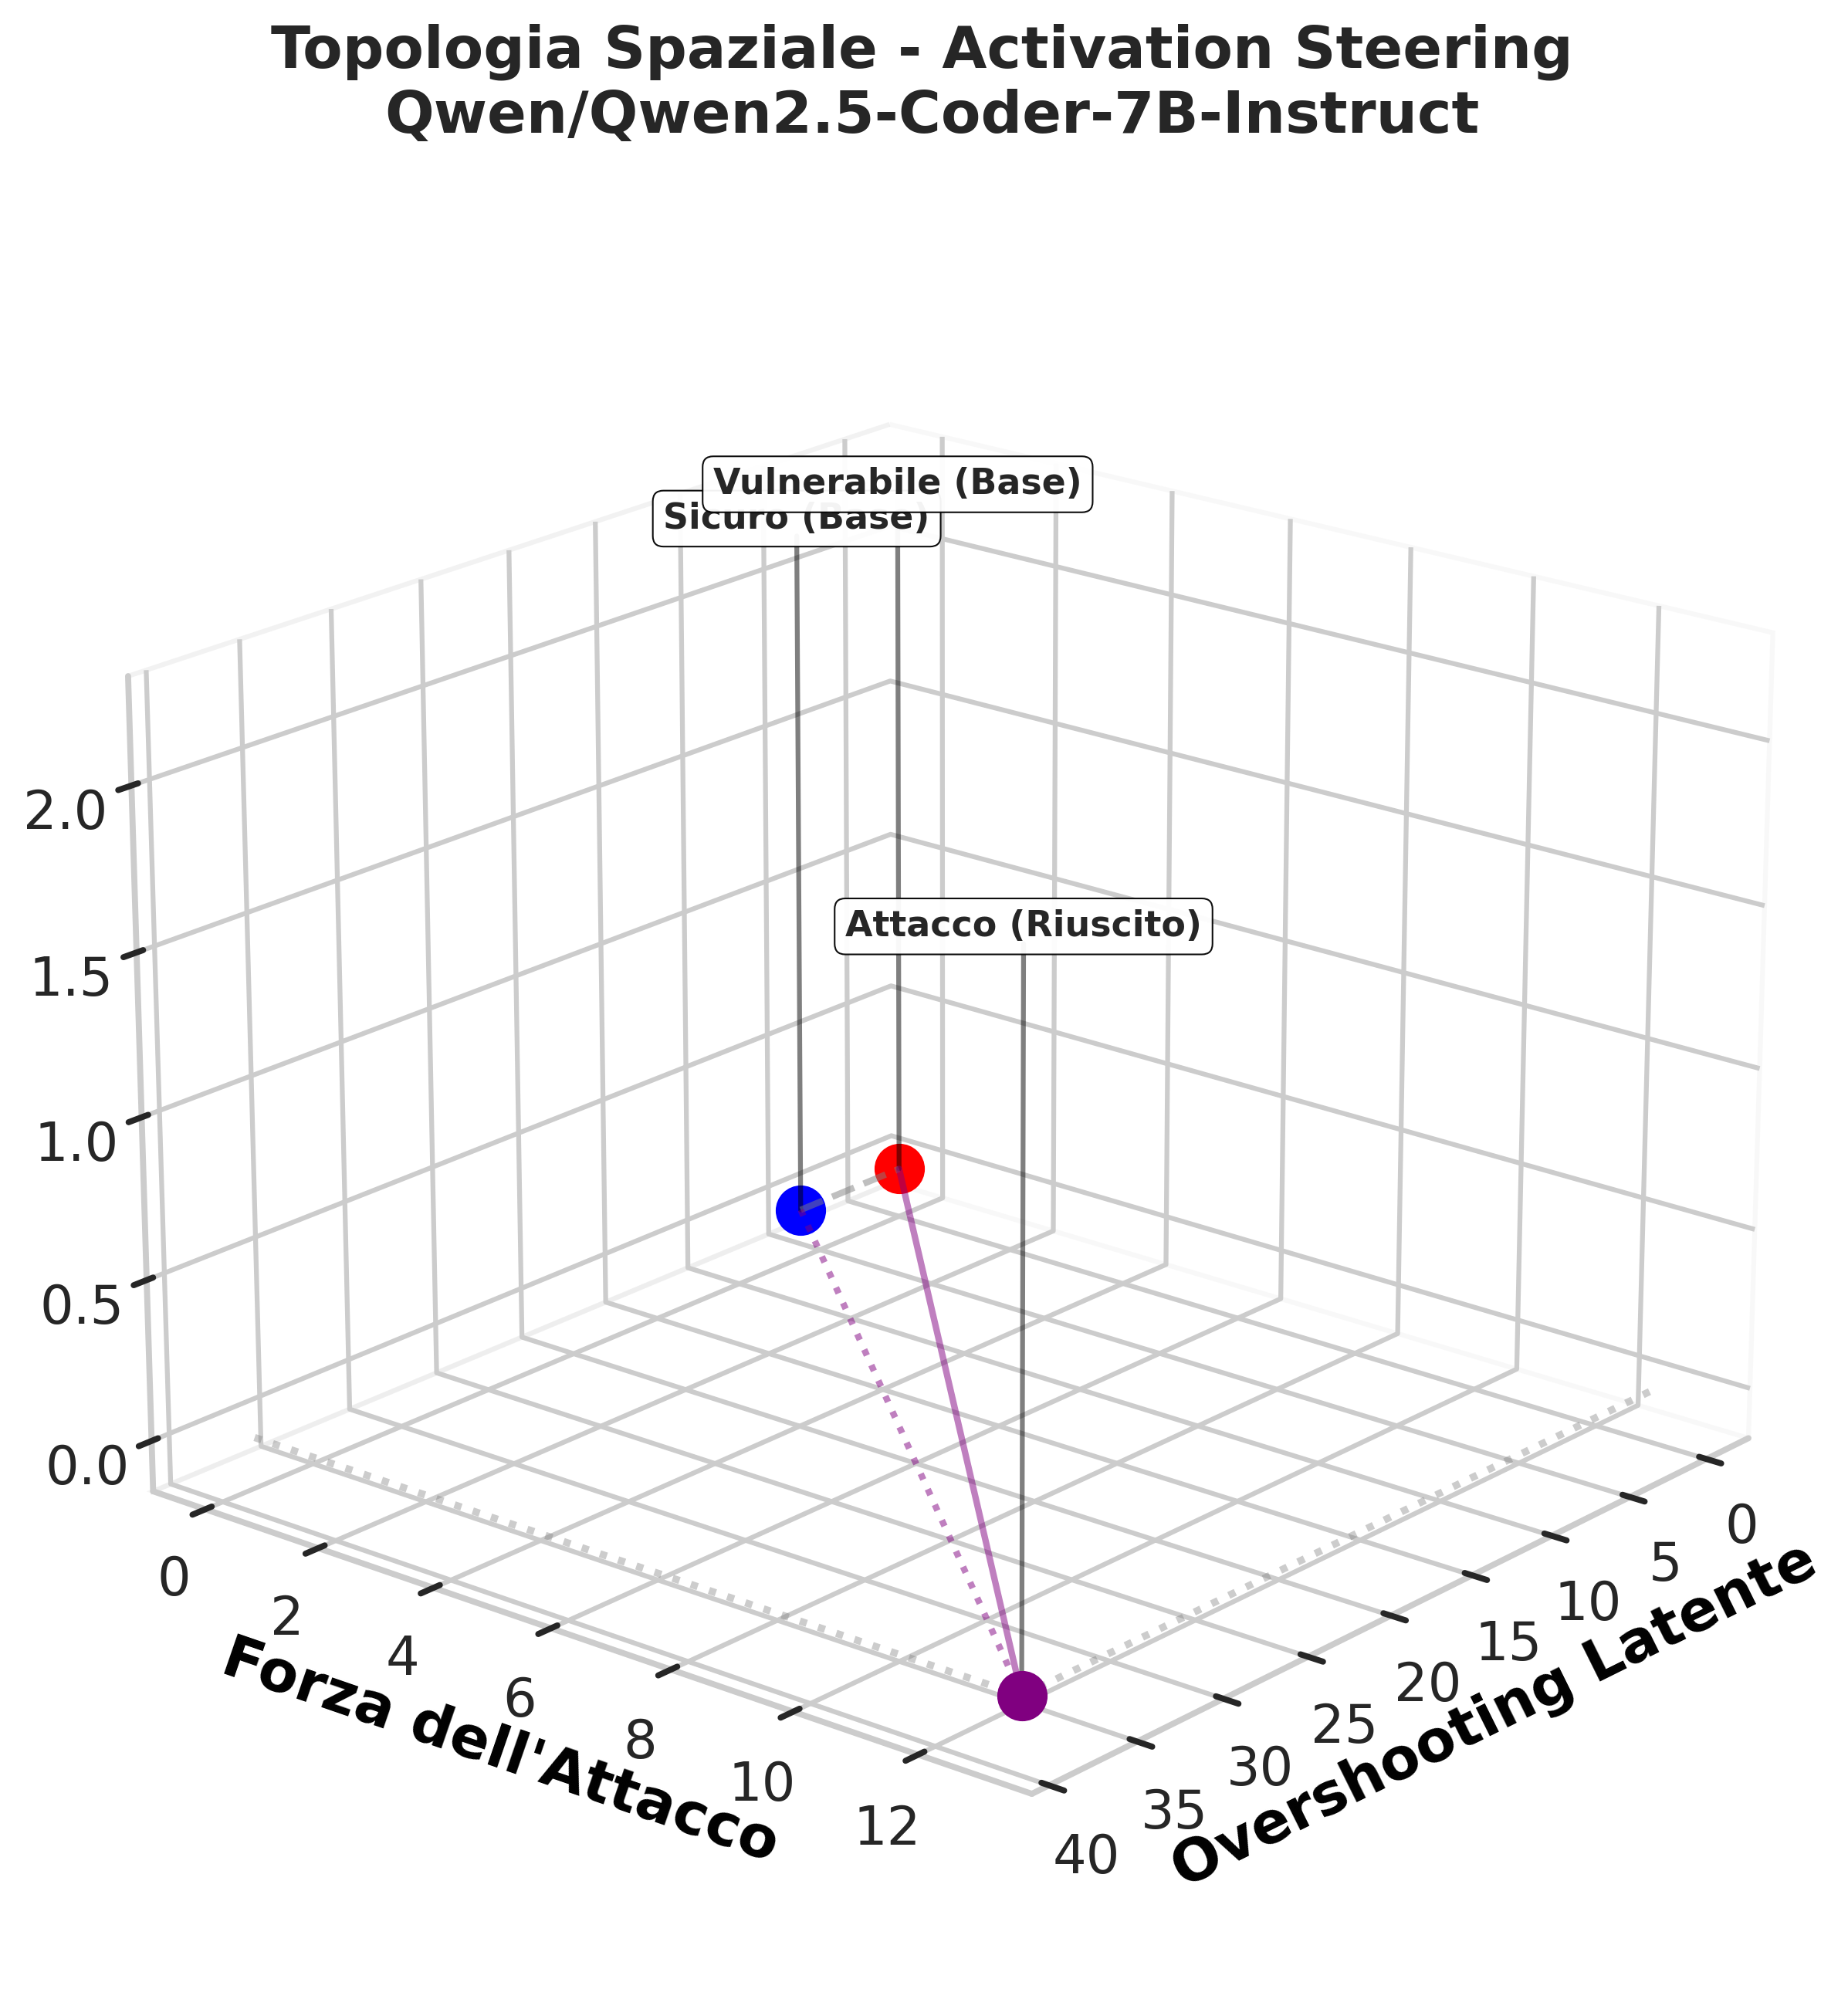
\includegraphics[width=\textwidth]{immagini/SWEEP L2/Steering_Topologia3D_Qwen_Qwen2.5-Coder-7B-Instruct_19.png}
        \caption{Qwen2.5-Coder-7B-Instruct}
    \end{subfigure}
\end{figure}

\begin{figure}[H]
    \centering
    \begin{subfigure}[b]{0.45\textwidth}
        \centering
        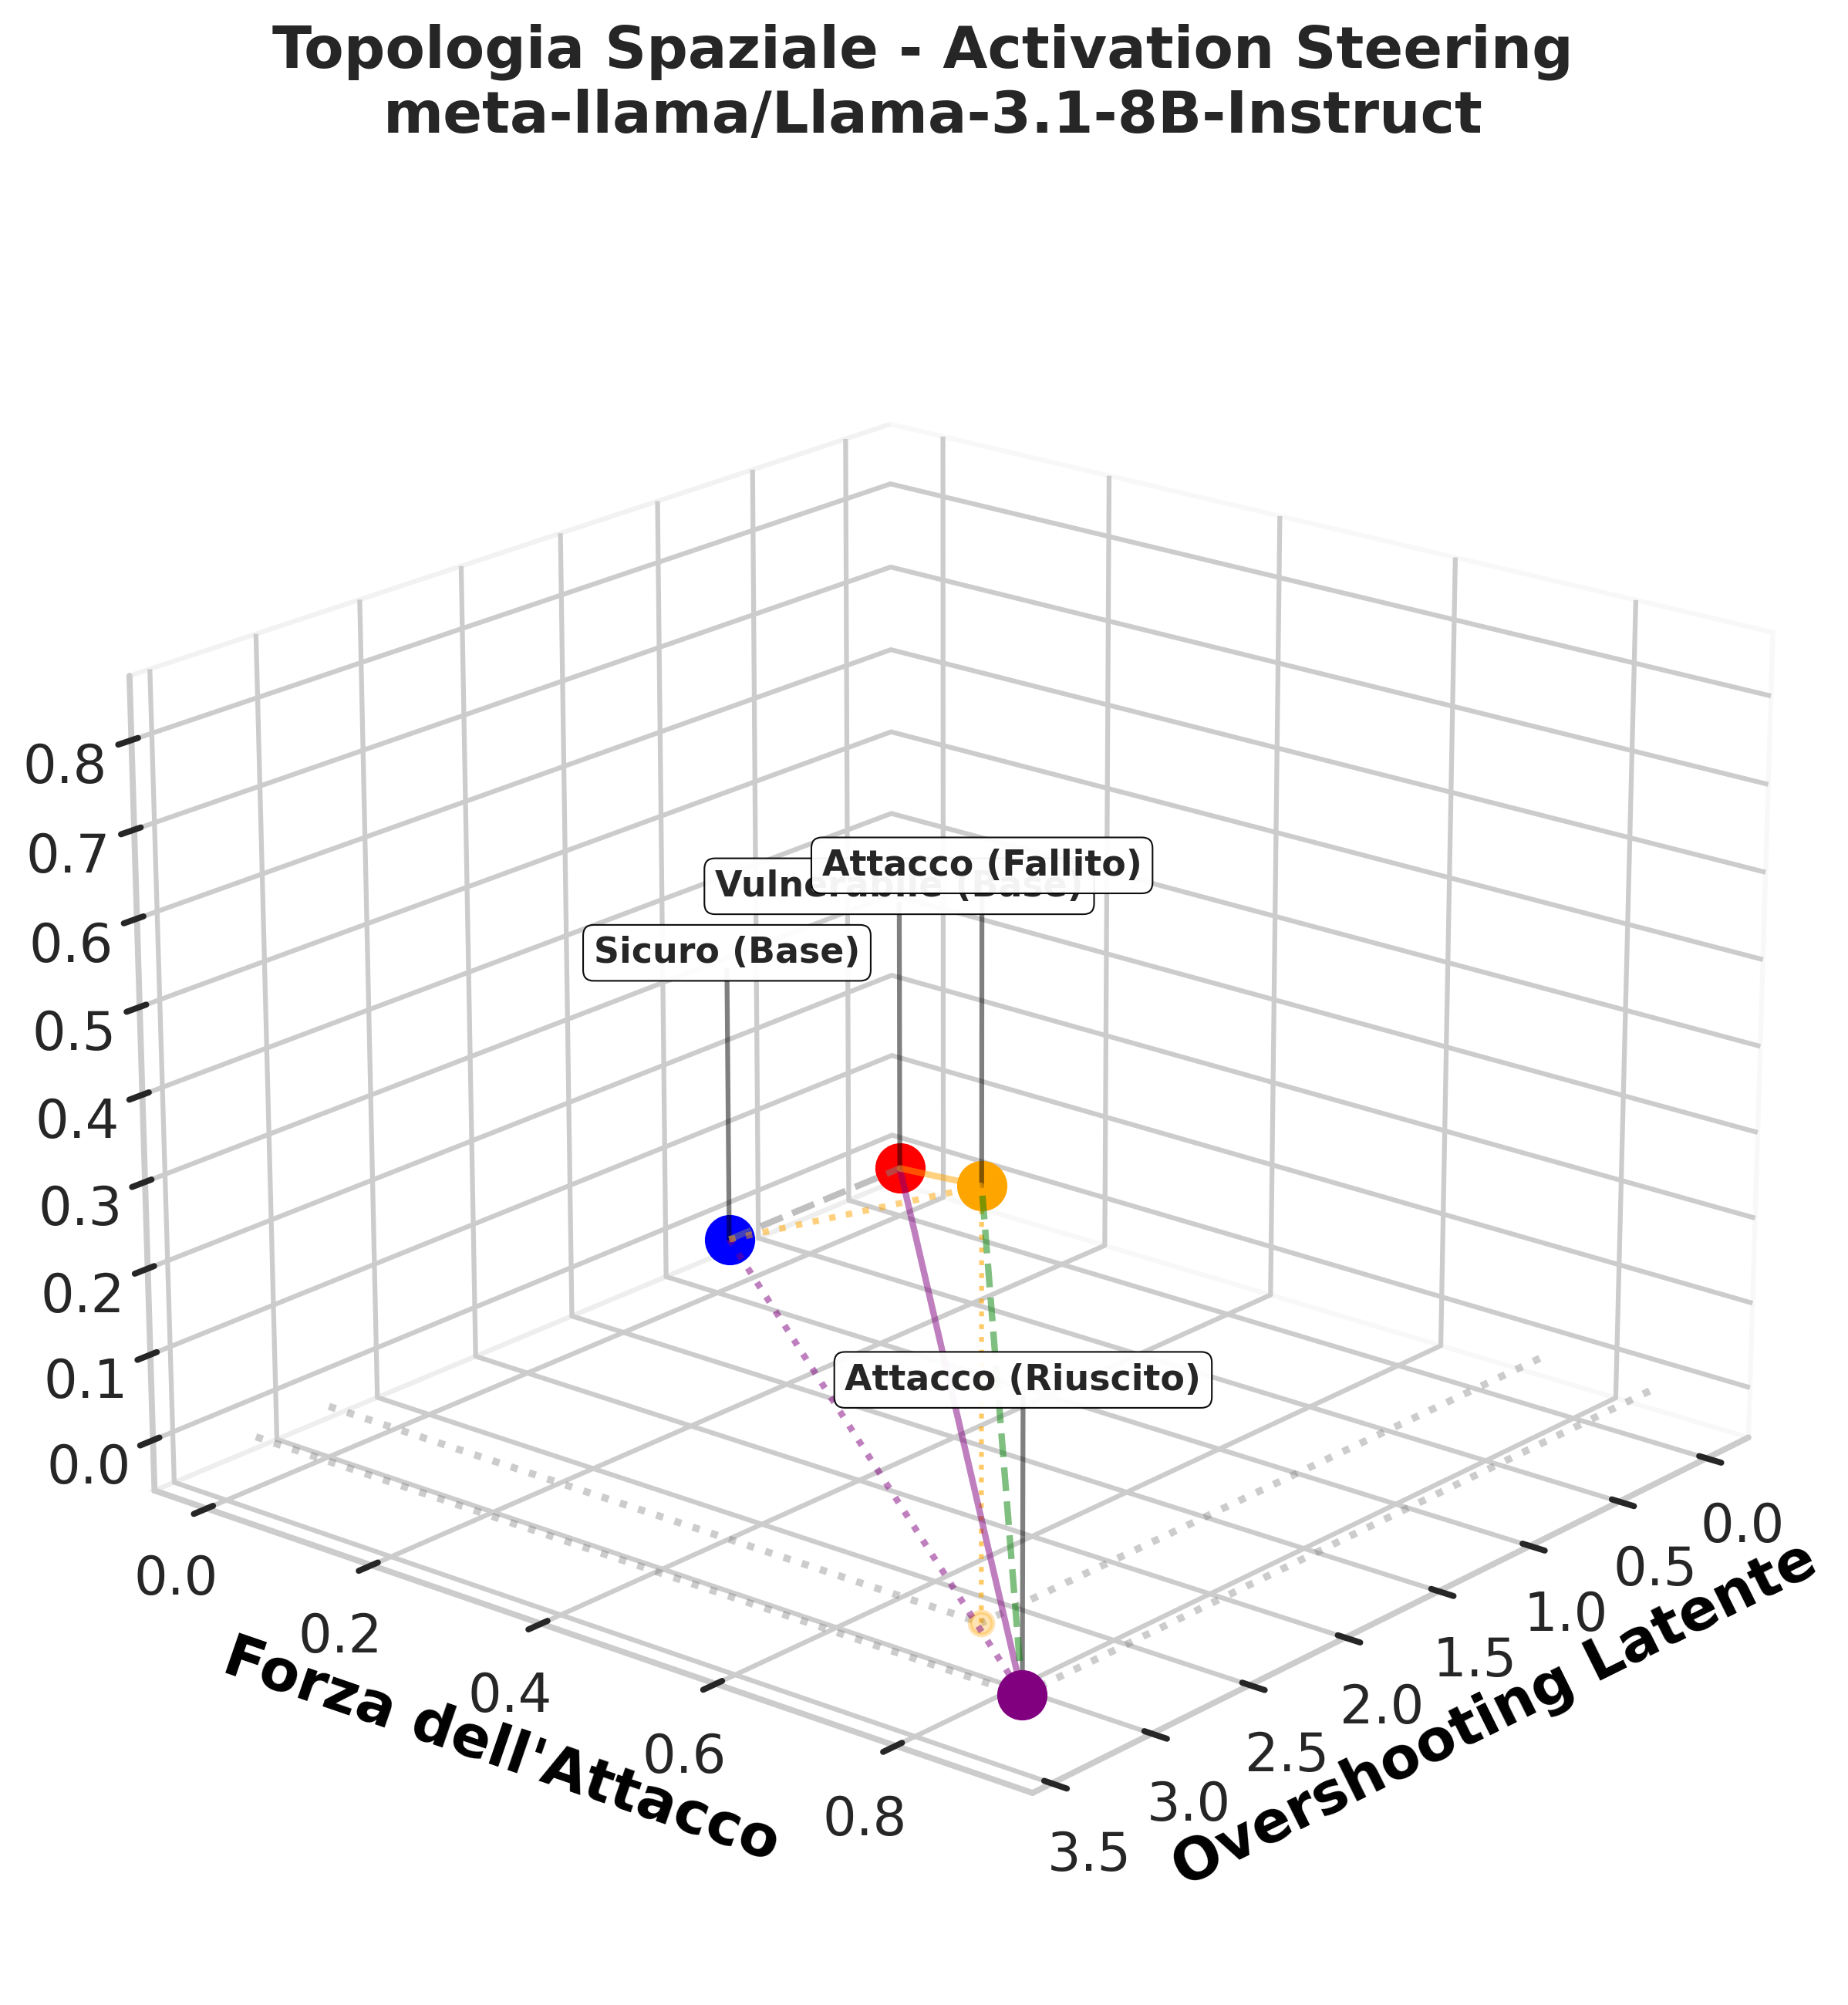
\includegraphics[width=\textwidth]{immagini/SWEEP L2/Steering_Topologia3D_meta-llama_Llama-3.1-8B-Instruct_16.png} 
        \caption{Llama-3.1-8B-Instruct}
    \end{subfigure}
    \hfill 
    \begin{subfigure}[b]{0.45\textwidth}
        \centering
        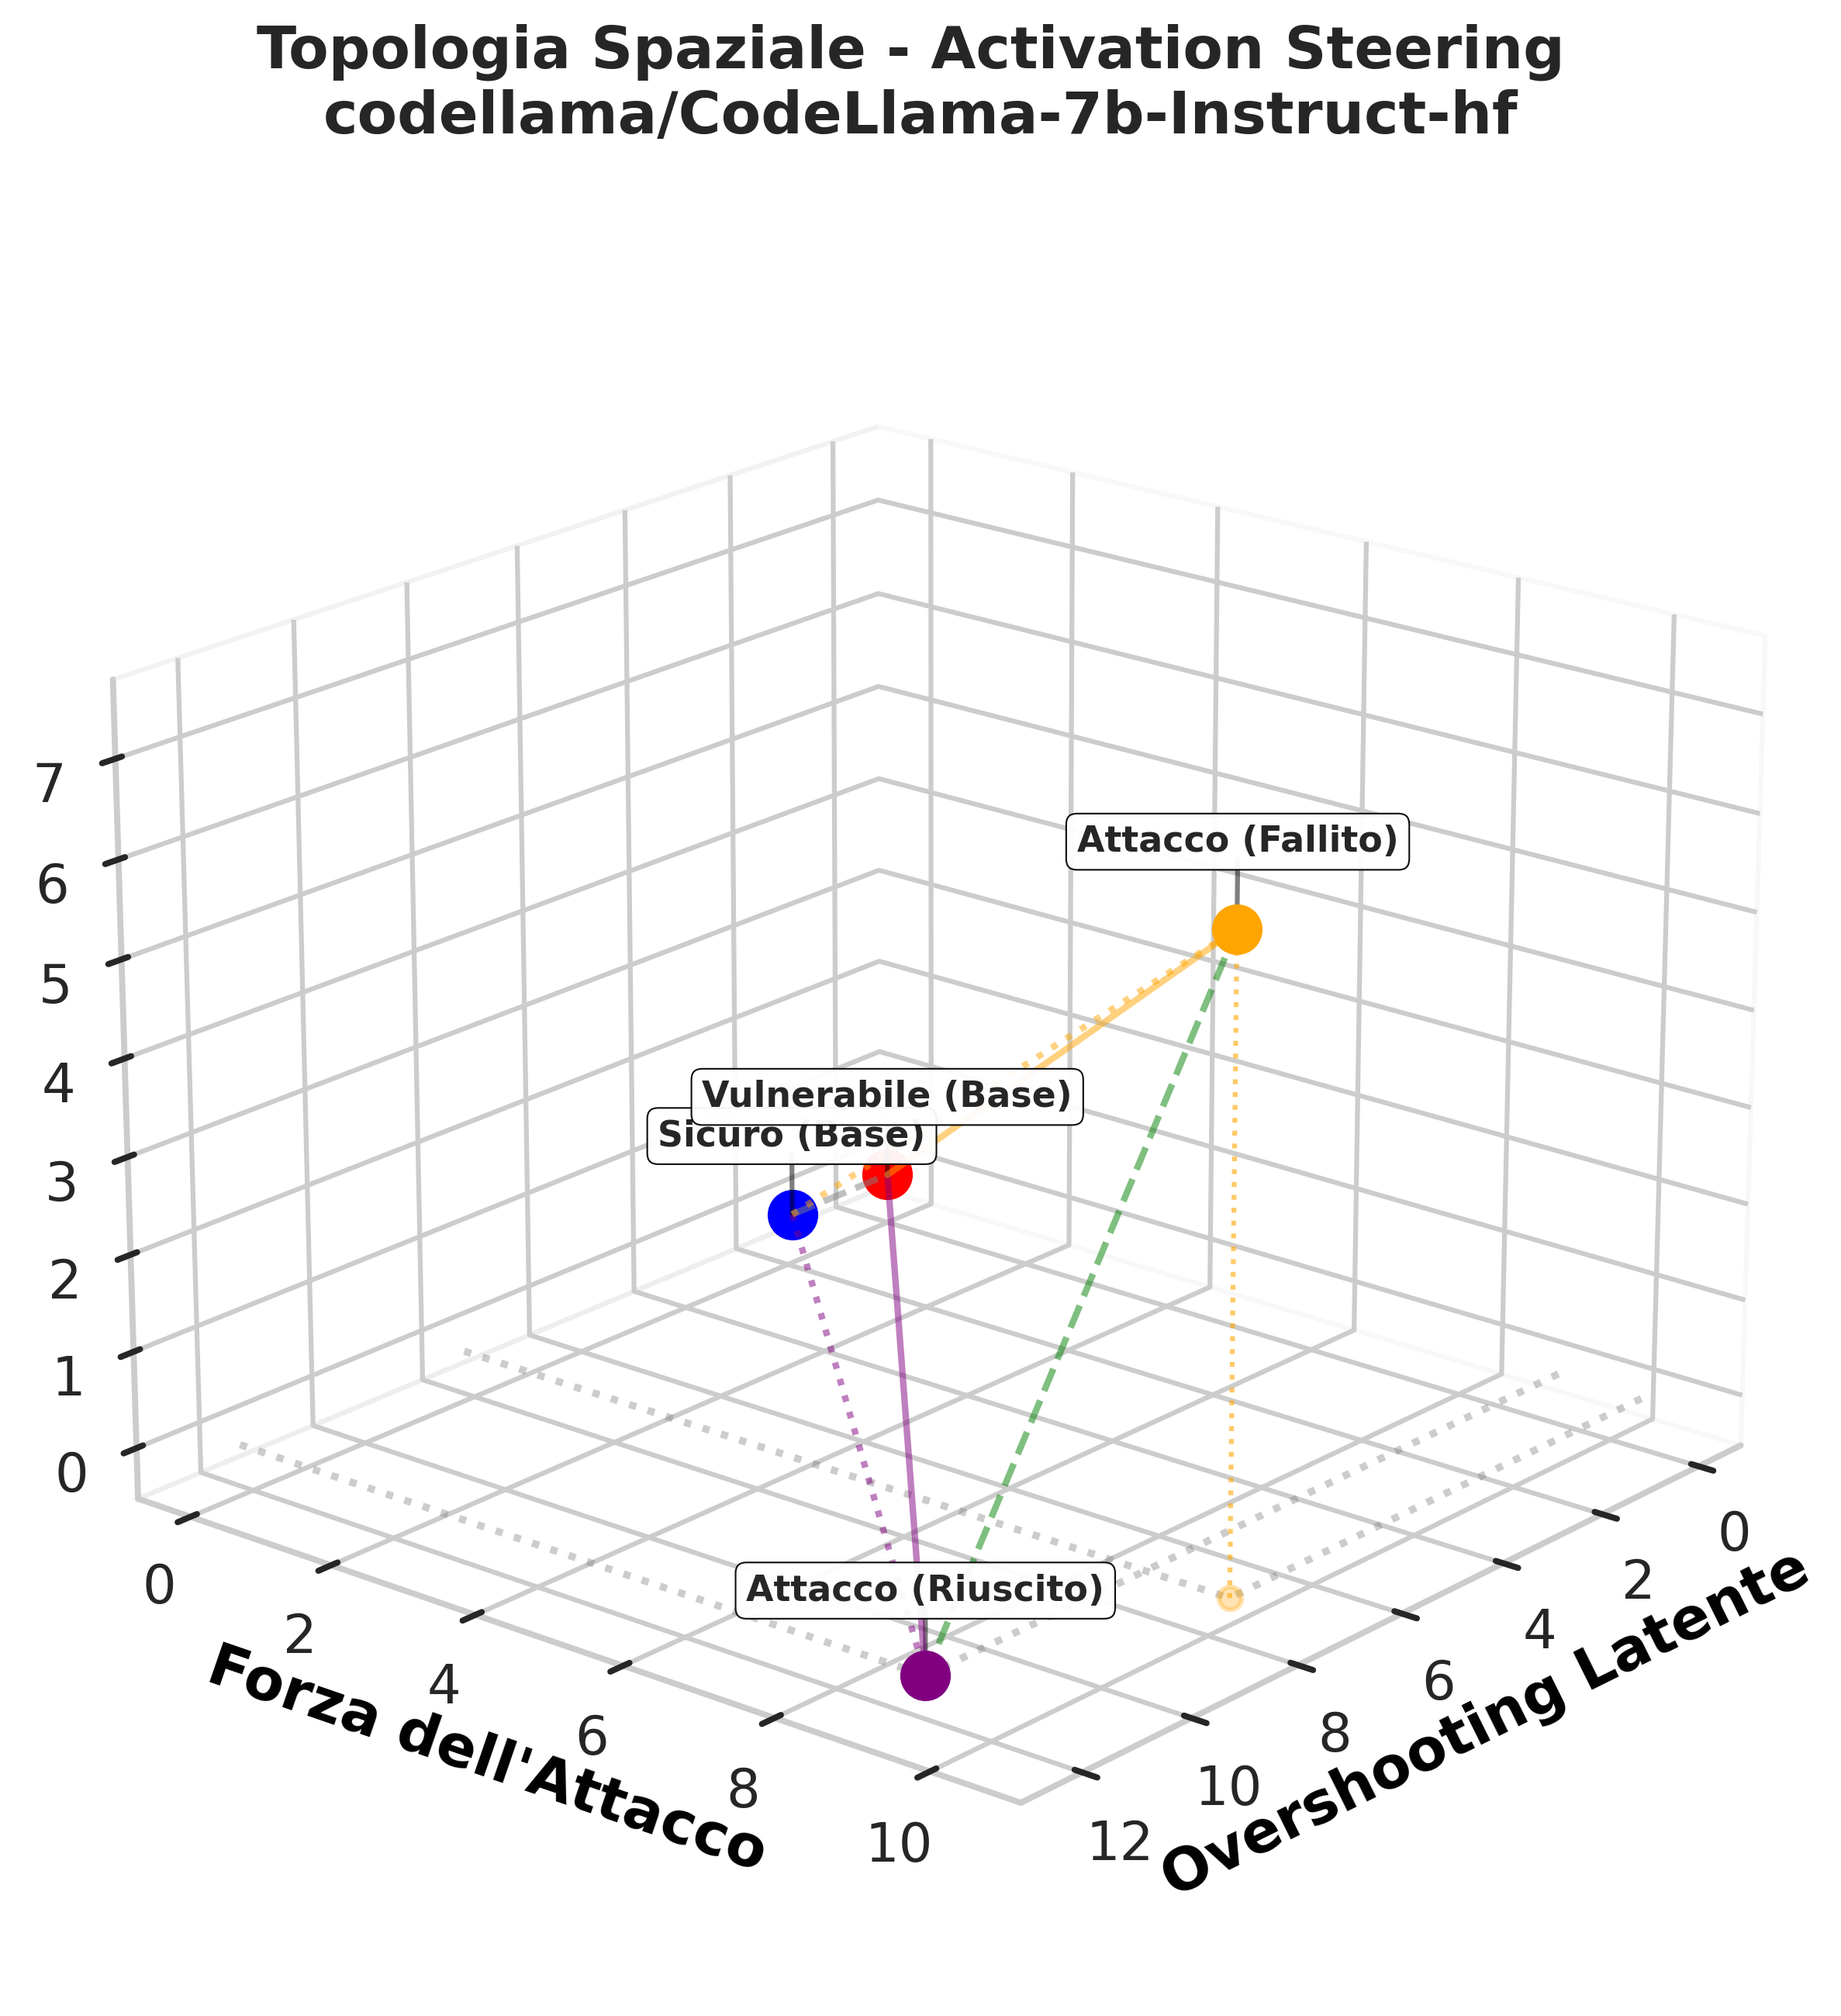
\includegraphics[width=\textwidth]{immagini/SWEEP L2/Steering_Topologia3D_codellama_CodeLlama-7b-Instruct-hf_14.png}
        \caption{CodeLlama-7b-Instruct-hf}
    \end{subfigure}
\end{figure}

\begin{figure}[H]
    \centering
    \begin{subfigure}[b]{0.45\textwidth}
        \centering
        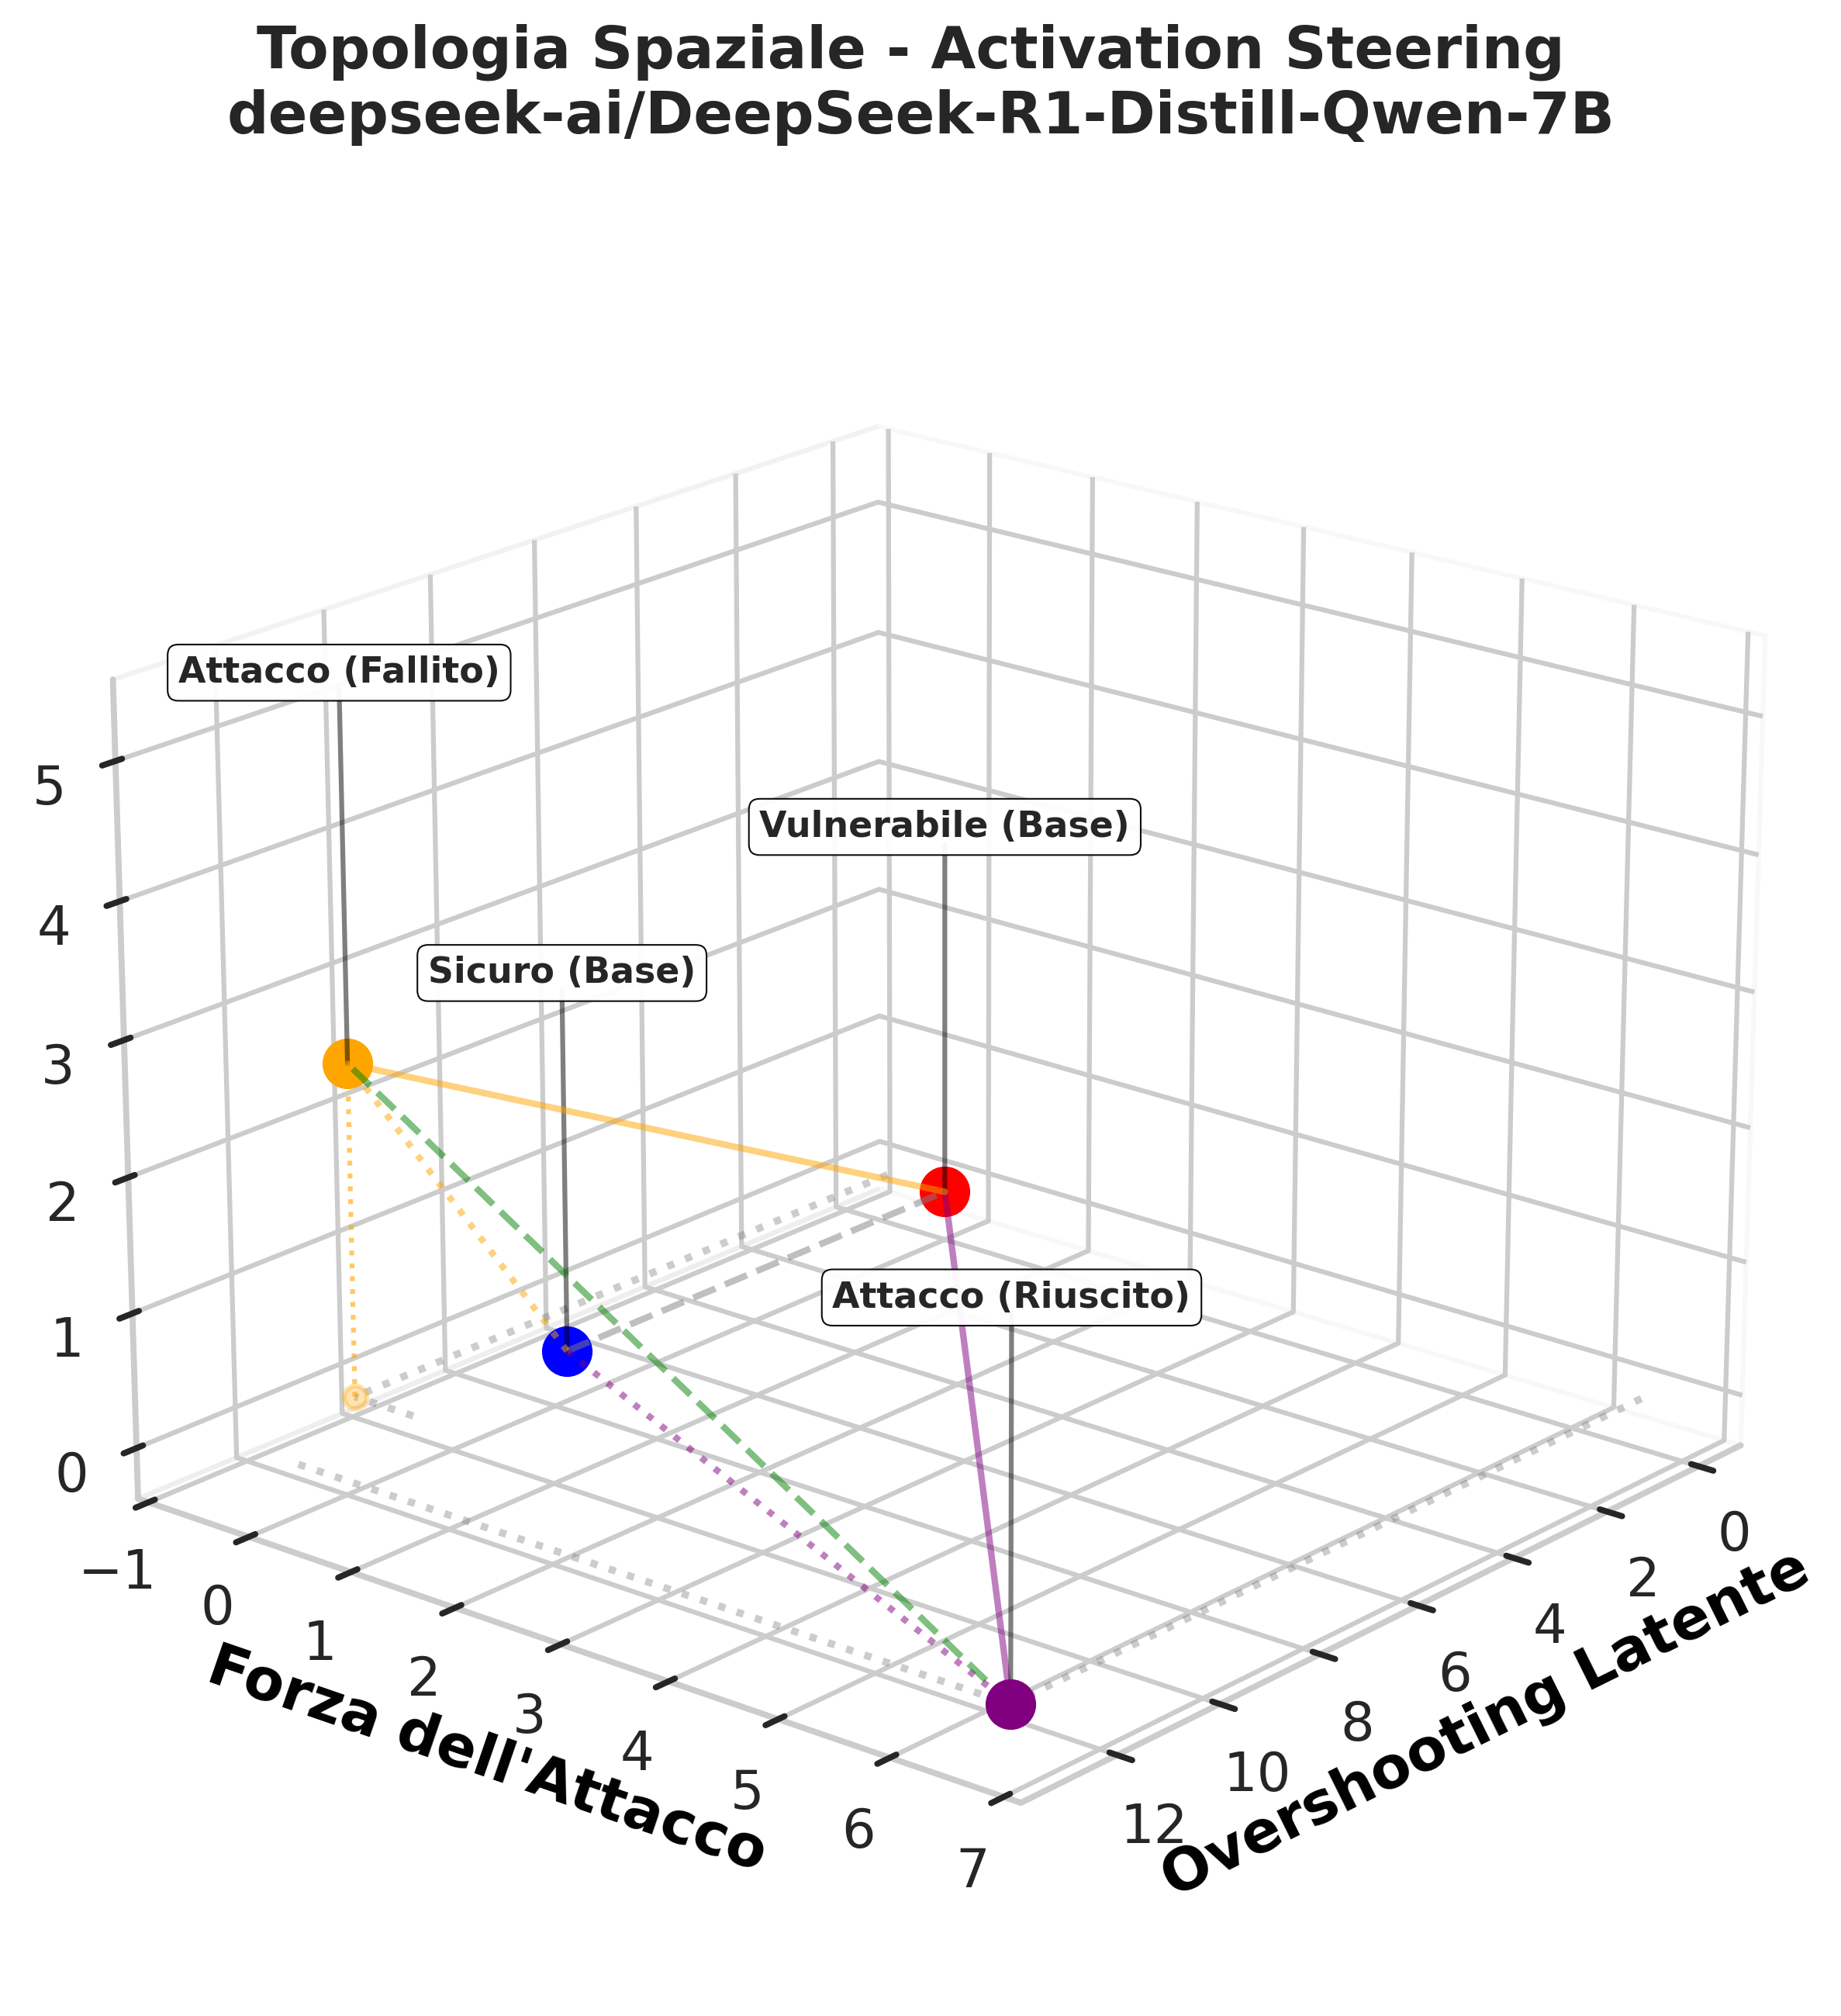
\includegraphics[width=\textwidth]{immagini/SWEEP L2/Steering_Topologia3D_deepseek-ai_DeepSeek-R1-Distill-Qwen-7B_20.png} 
        \caption{DeepSeek-R1-Distill-Qwen-7B}
    \end{subfigure}
    \hfill 
    \begin{subfigure}[b]{0.45\textwidth}
        \centering
        
\includegraphics[width=\textwidth]{immagini/SWEEP L2/Steering_Topologia3D_deepseek-ai_deepseek-coder-6.7b-instruct_17.png}
        \caption{deepseek-coder-6.7b-instruct}
    \end{subfigure}
\end{figure}

\newpage

\section{Evoluzione delle distanze}
Vengono presentati i grafici relativi all'evoluzione delle distanze L2 per tutti i layer dei modelli

\begin{figure}[H]
    \centering
    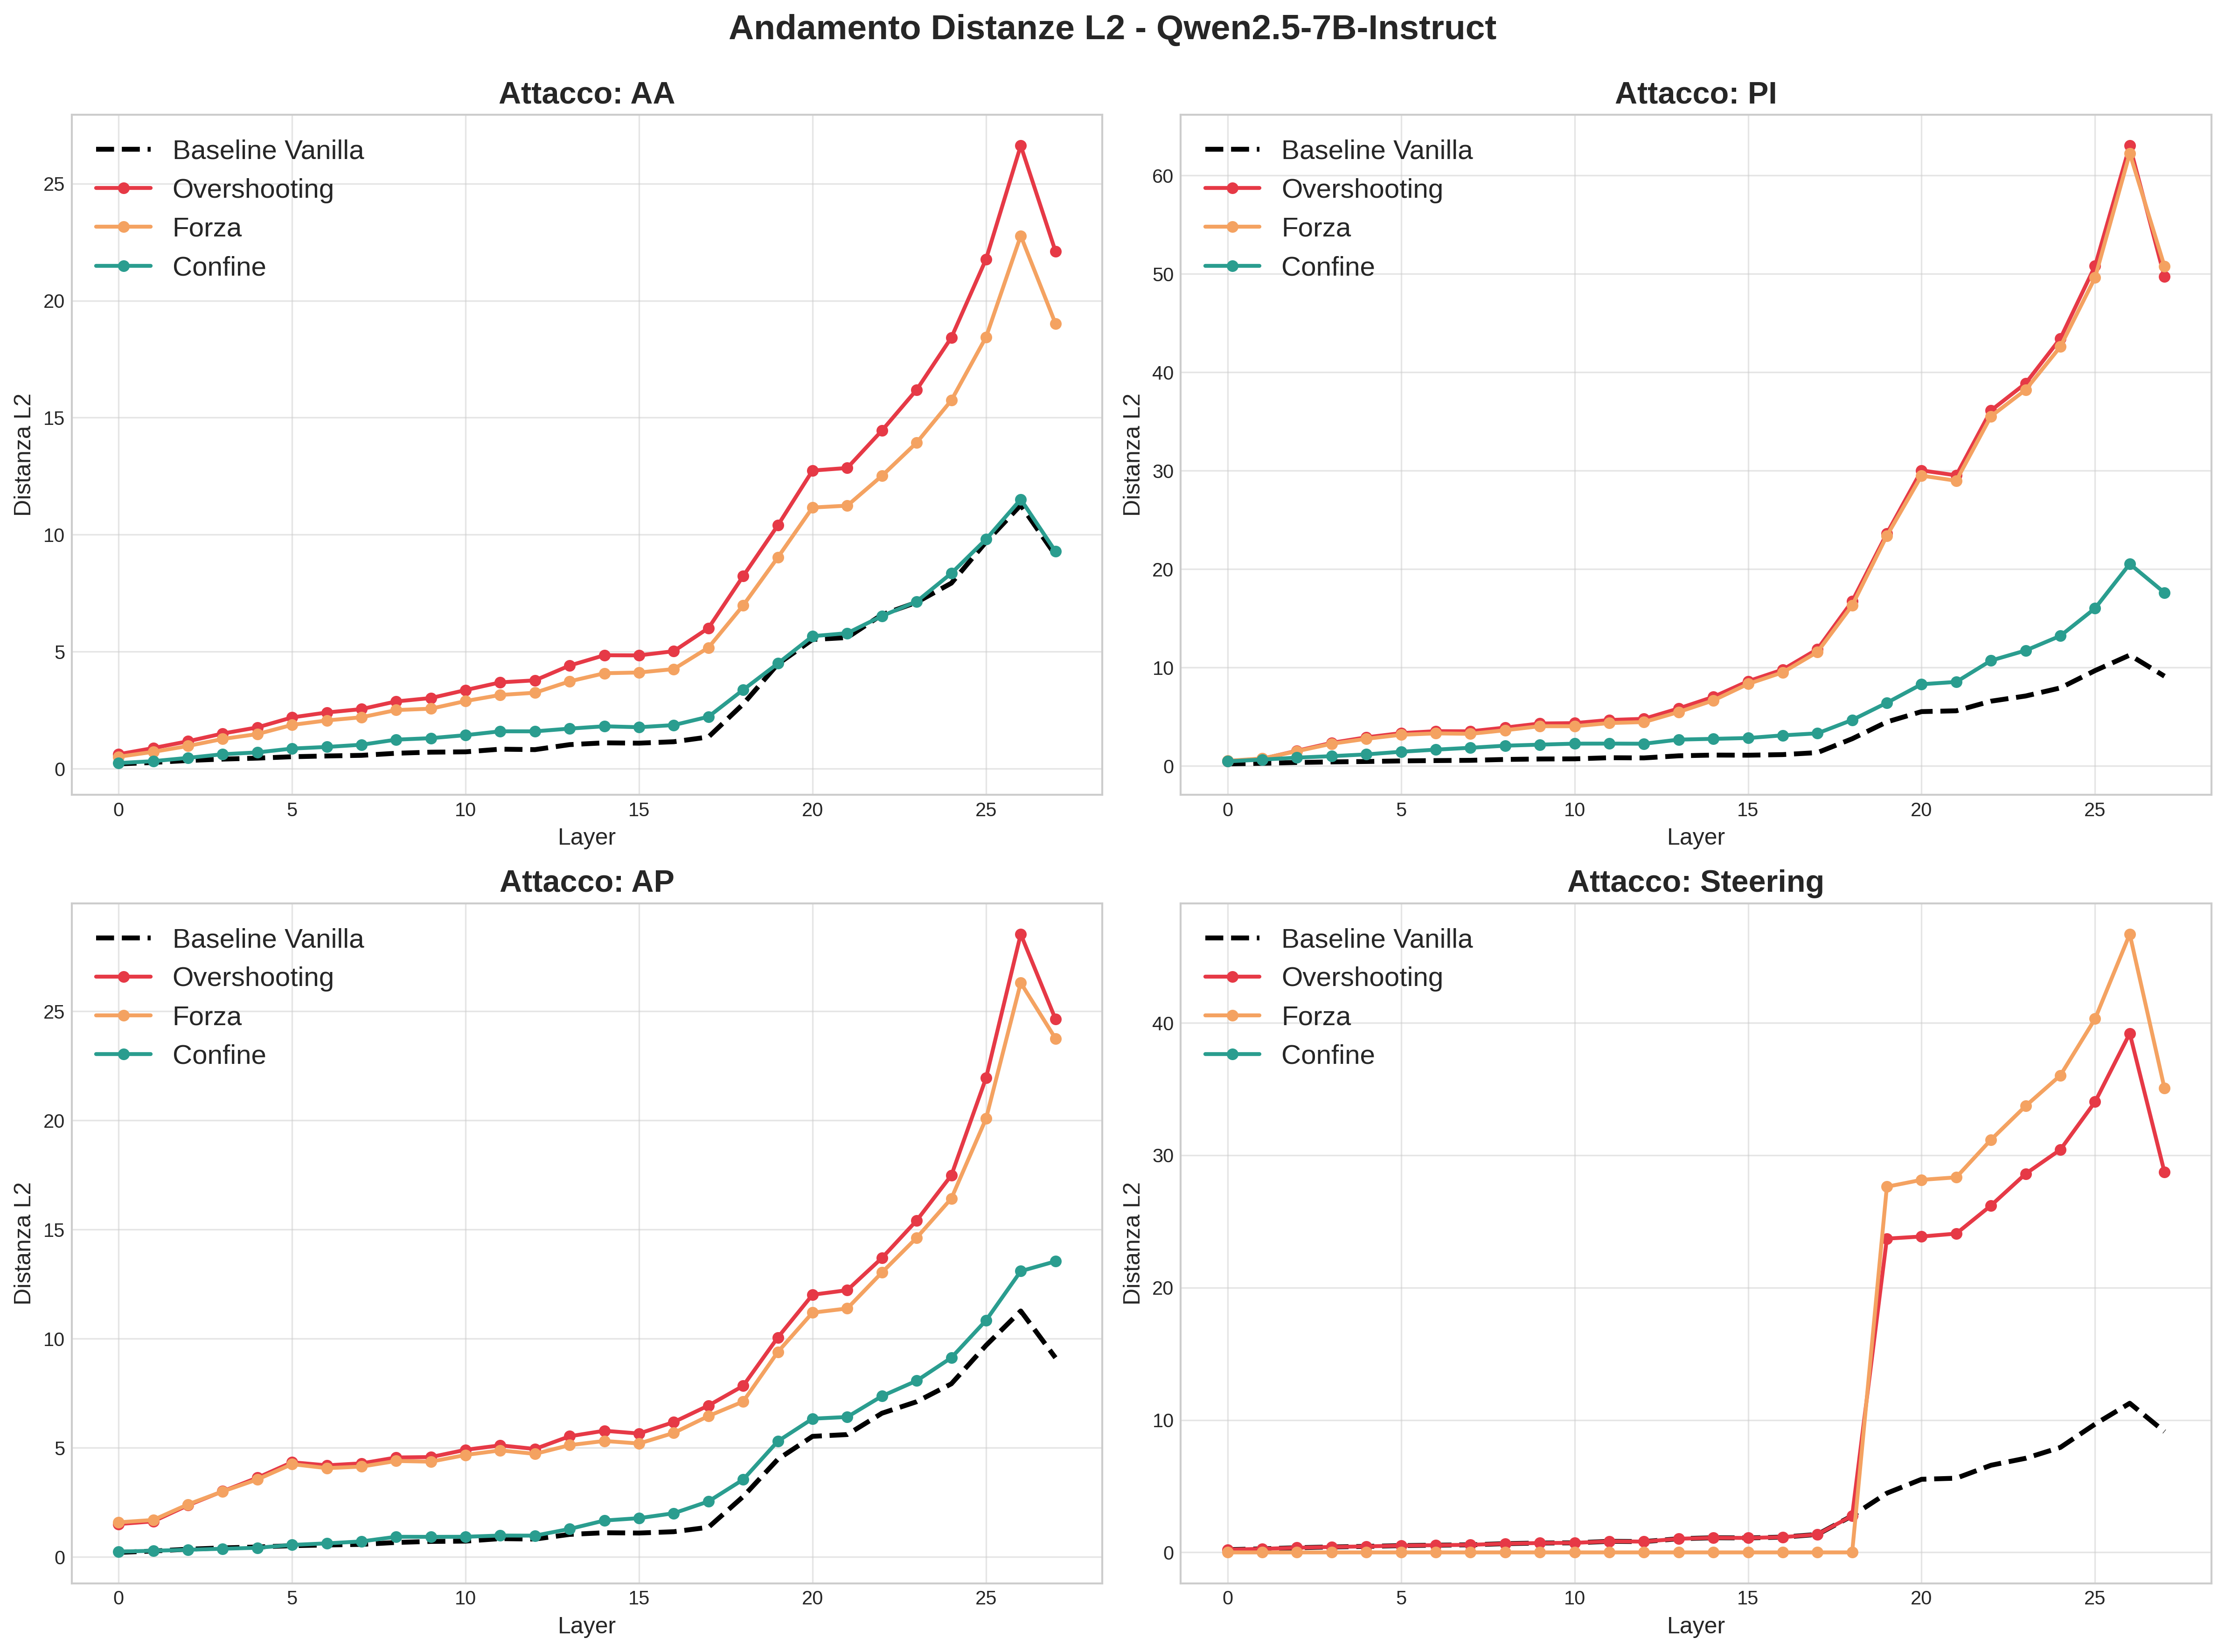
\includegraphics[width=\textwidth]{immagini/anda/Qwen2.5-7B-Instruct_L2_Trends.png}
\end{figure}

\begin{figure}[H]
    \centering
    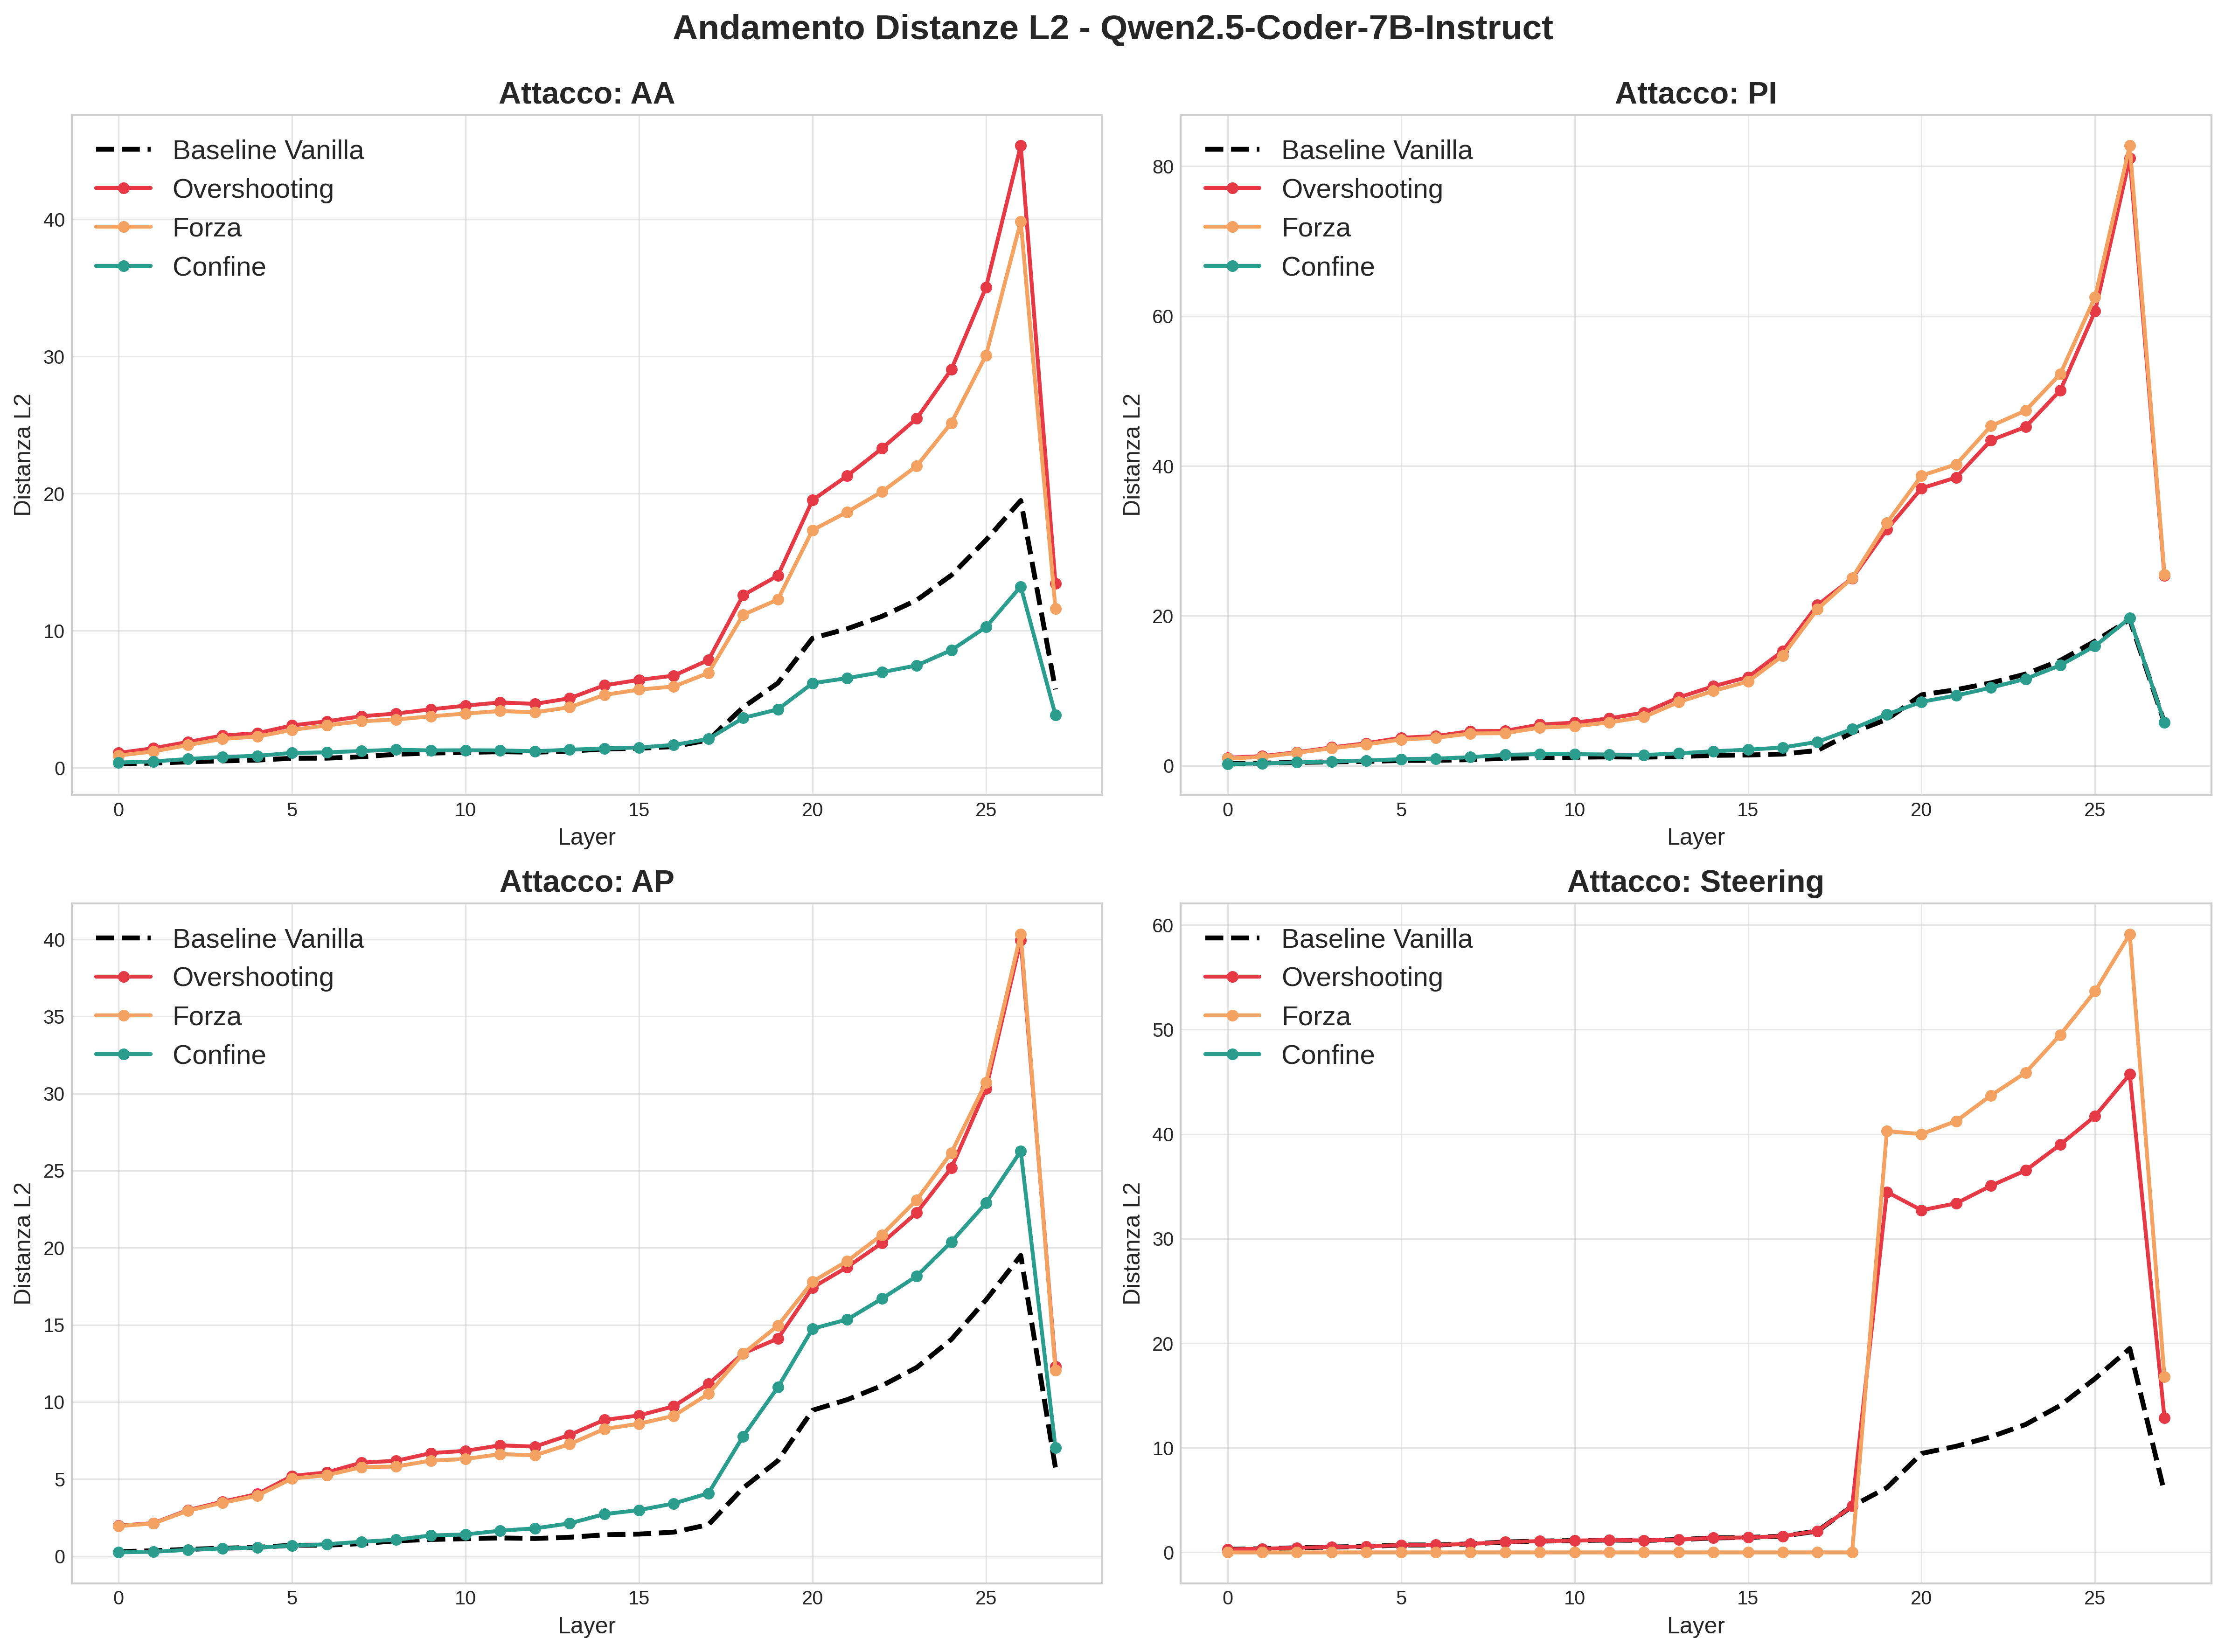
\includegraphics[width=\textwidth]{immagini/anda/Qwen2.5-Coder-7B-Instruct_L2_Trends.png}
\end{figure}

\begin{figure}[H]
    \centering
    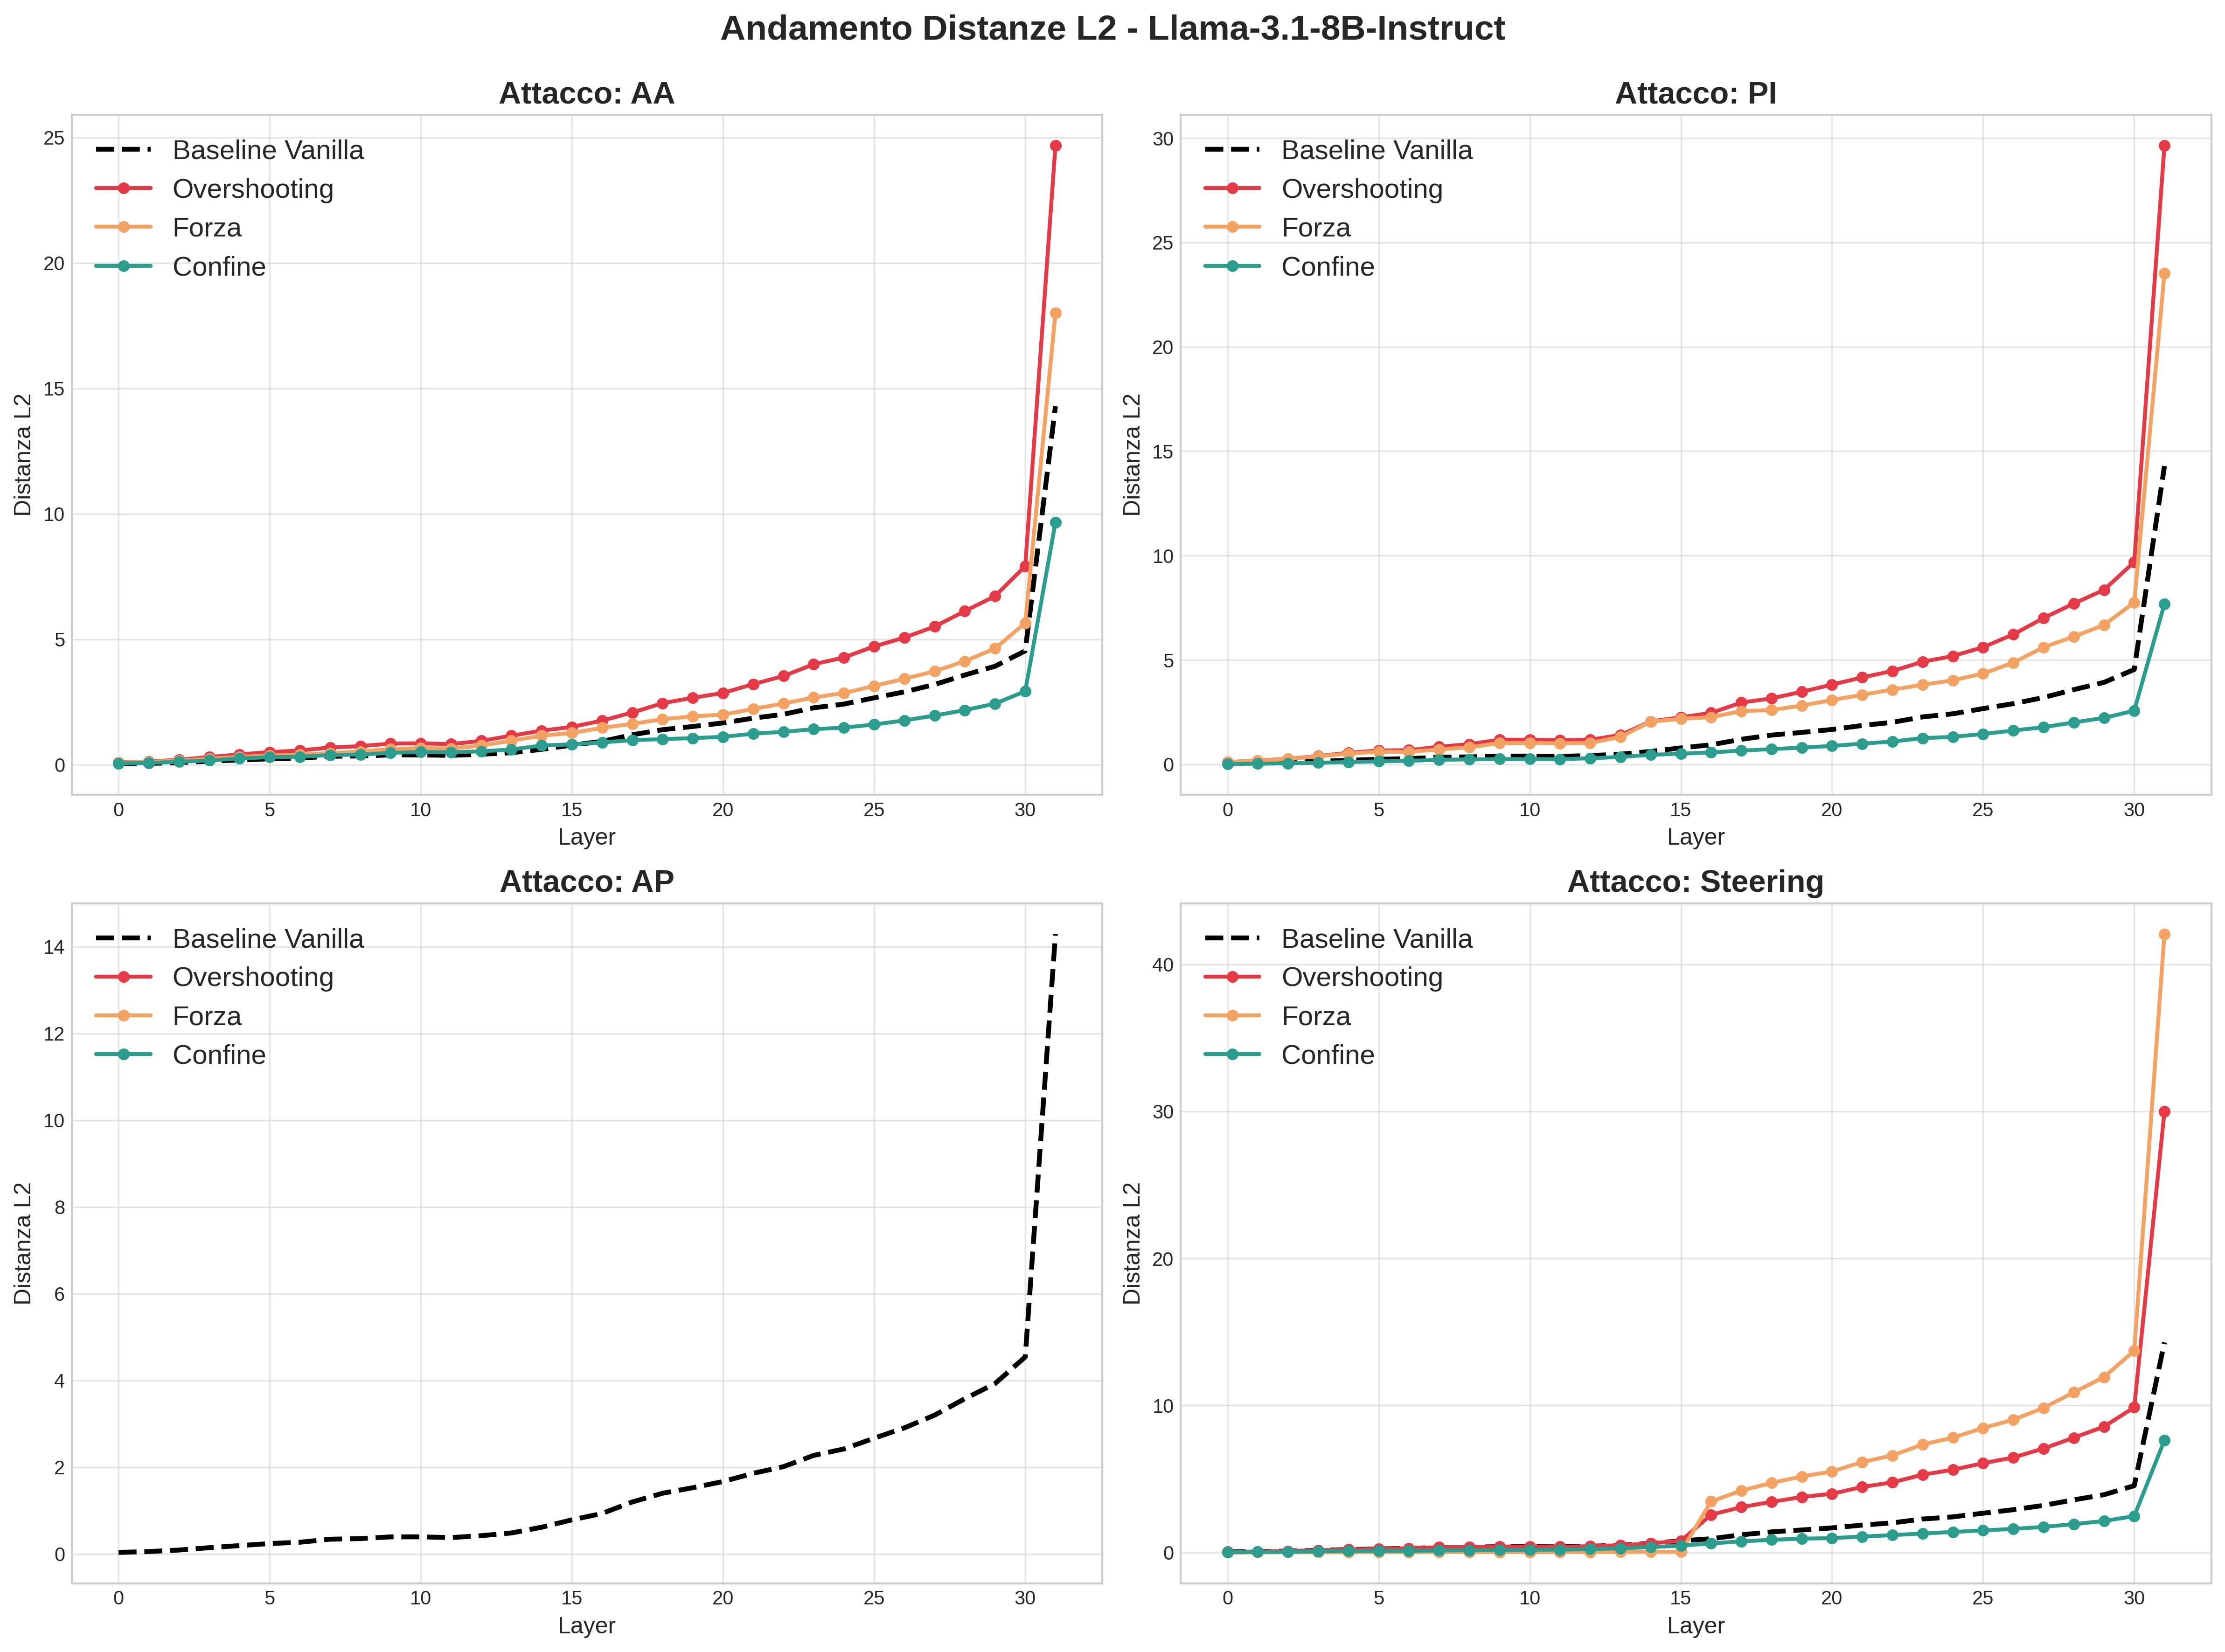
\includegraphics[width=\textwidth]{immagini/anda/Llama-3.1-8B-Instruct_L2_Trends.png}
\end{figure}

\begin{figure}[H]
    \centering
    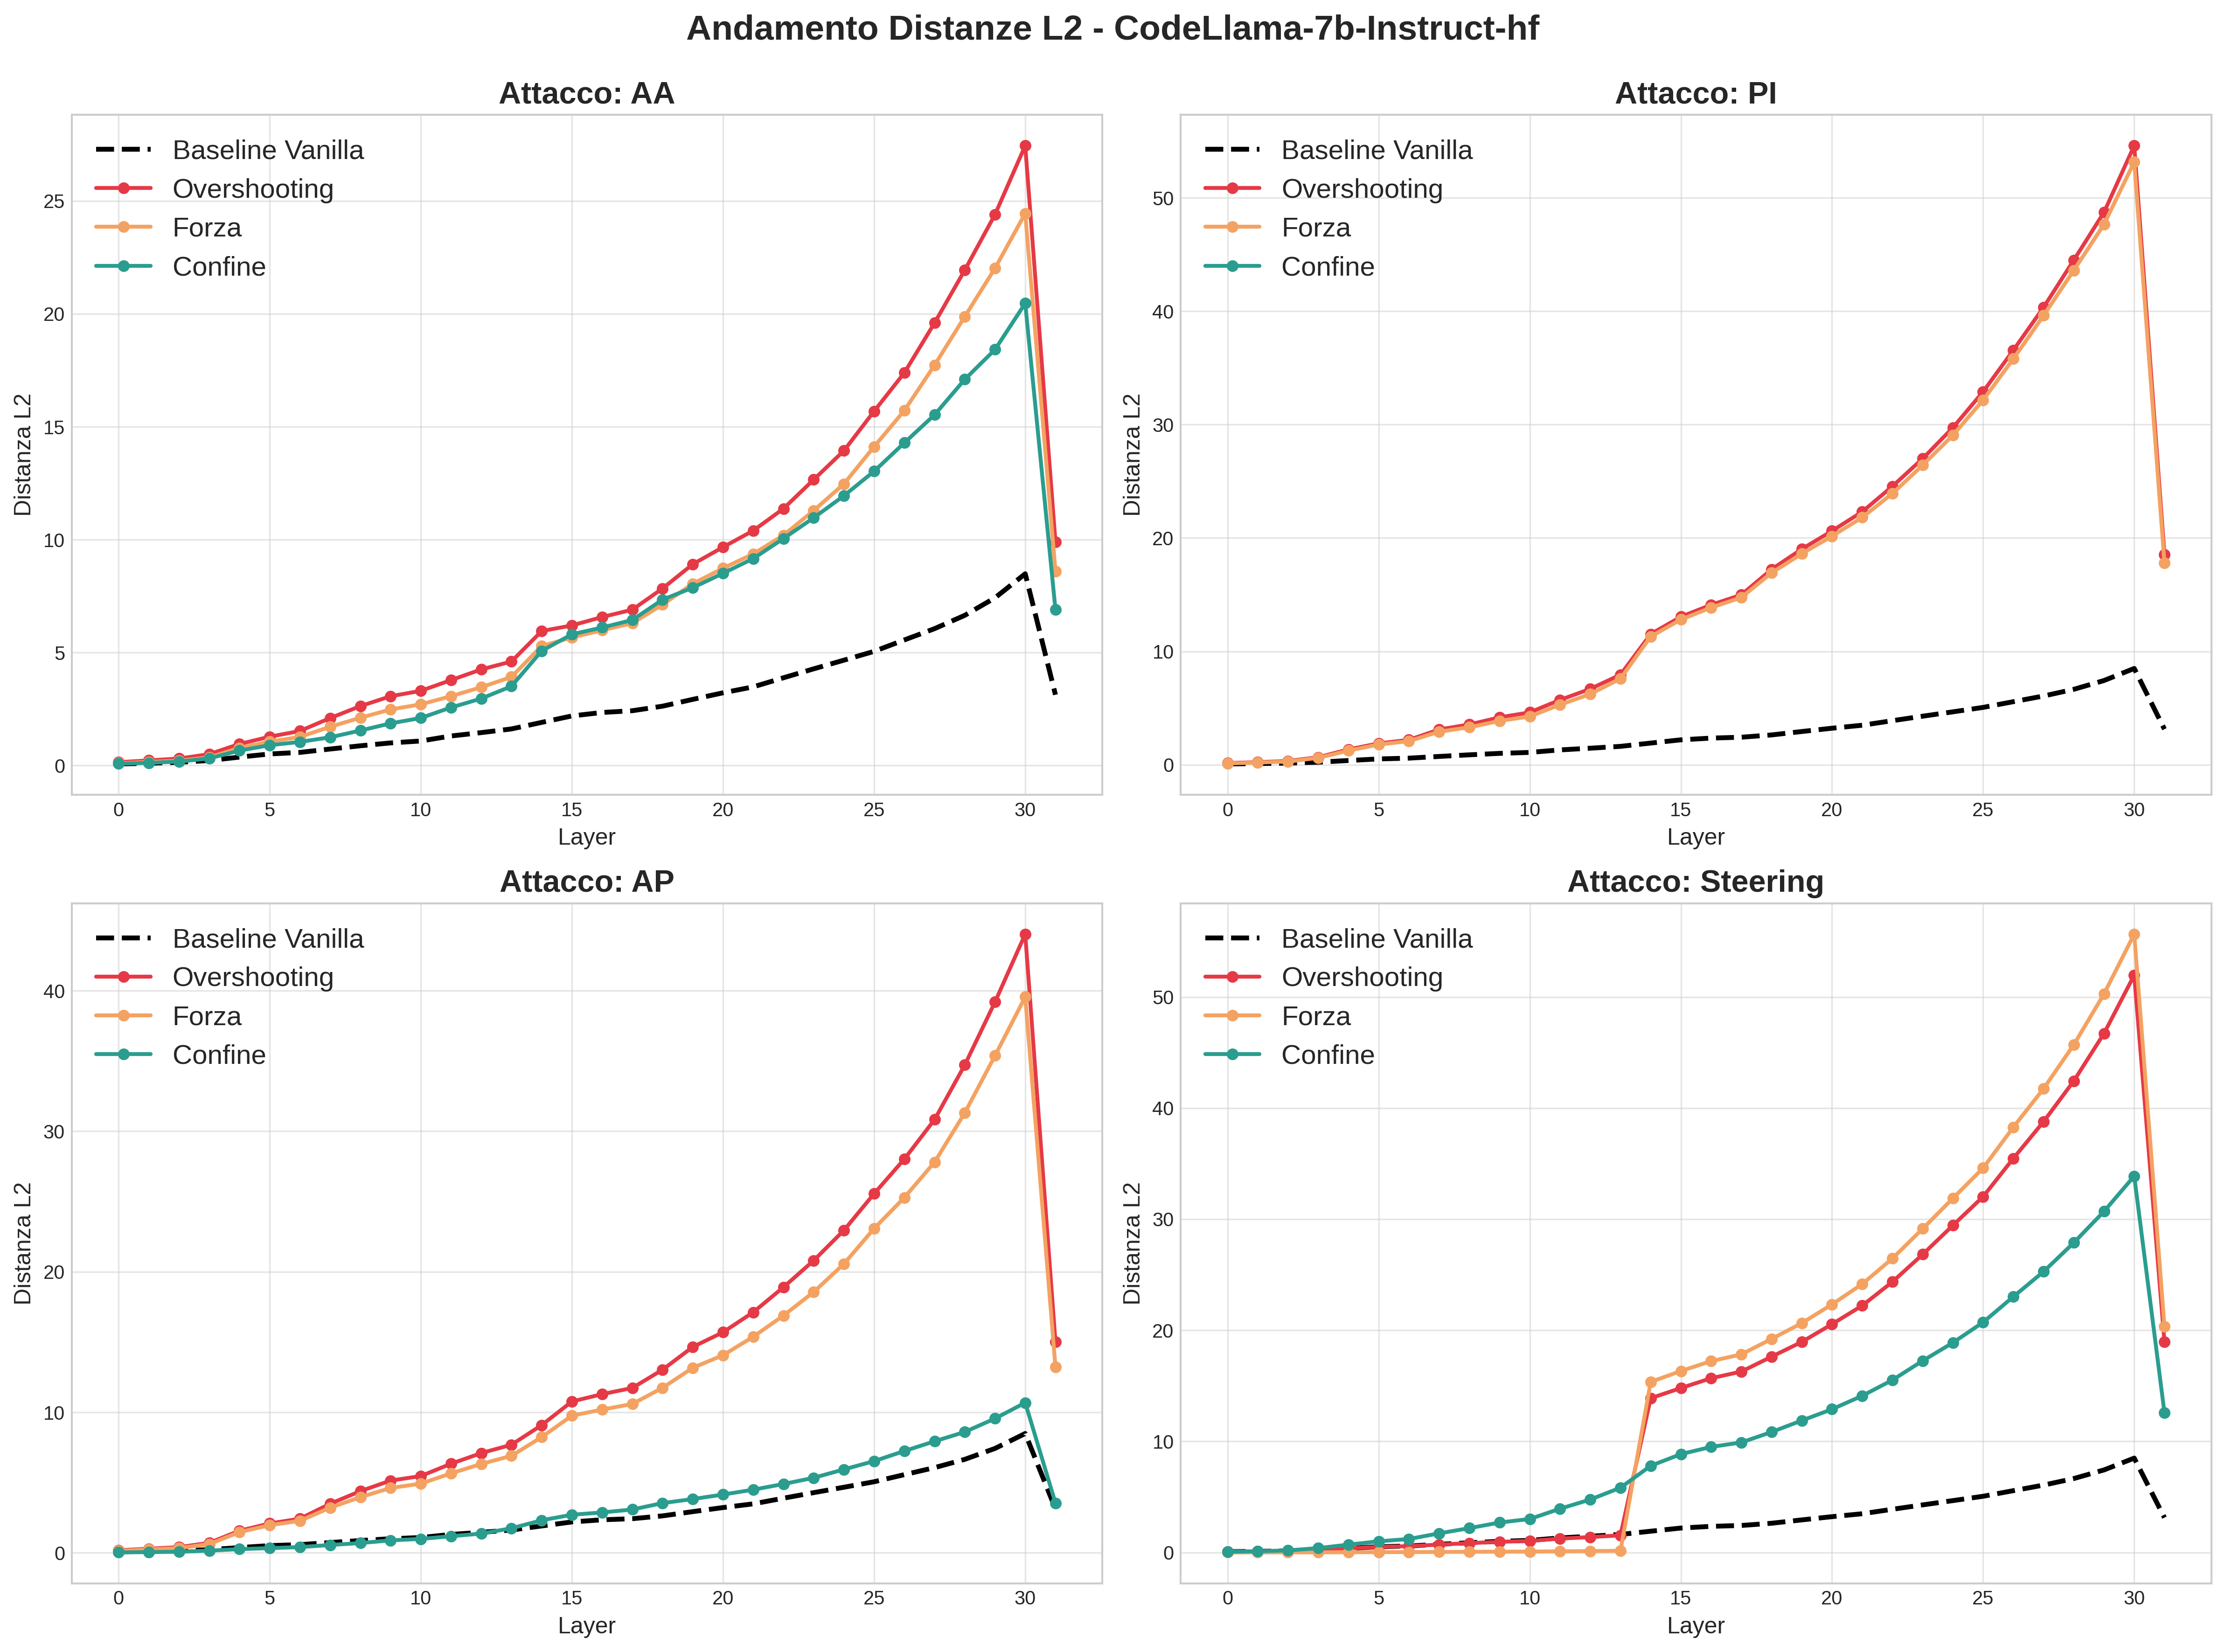
\includegraphics[width=\textwidth]{immagini/anda/CodeLlama-7b-Instruct-hf_L2_Trends.png}
\end{figure}

\begin{figure}[H]
    \centering
    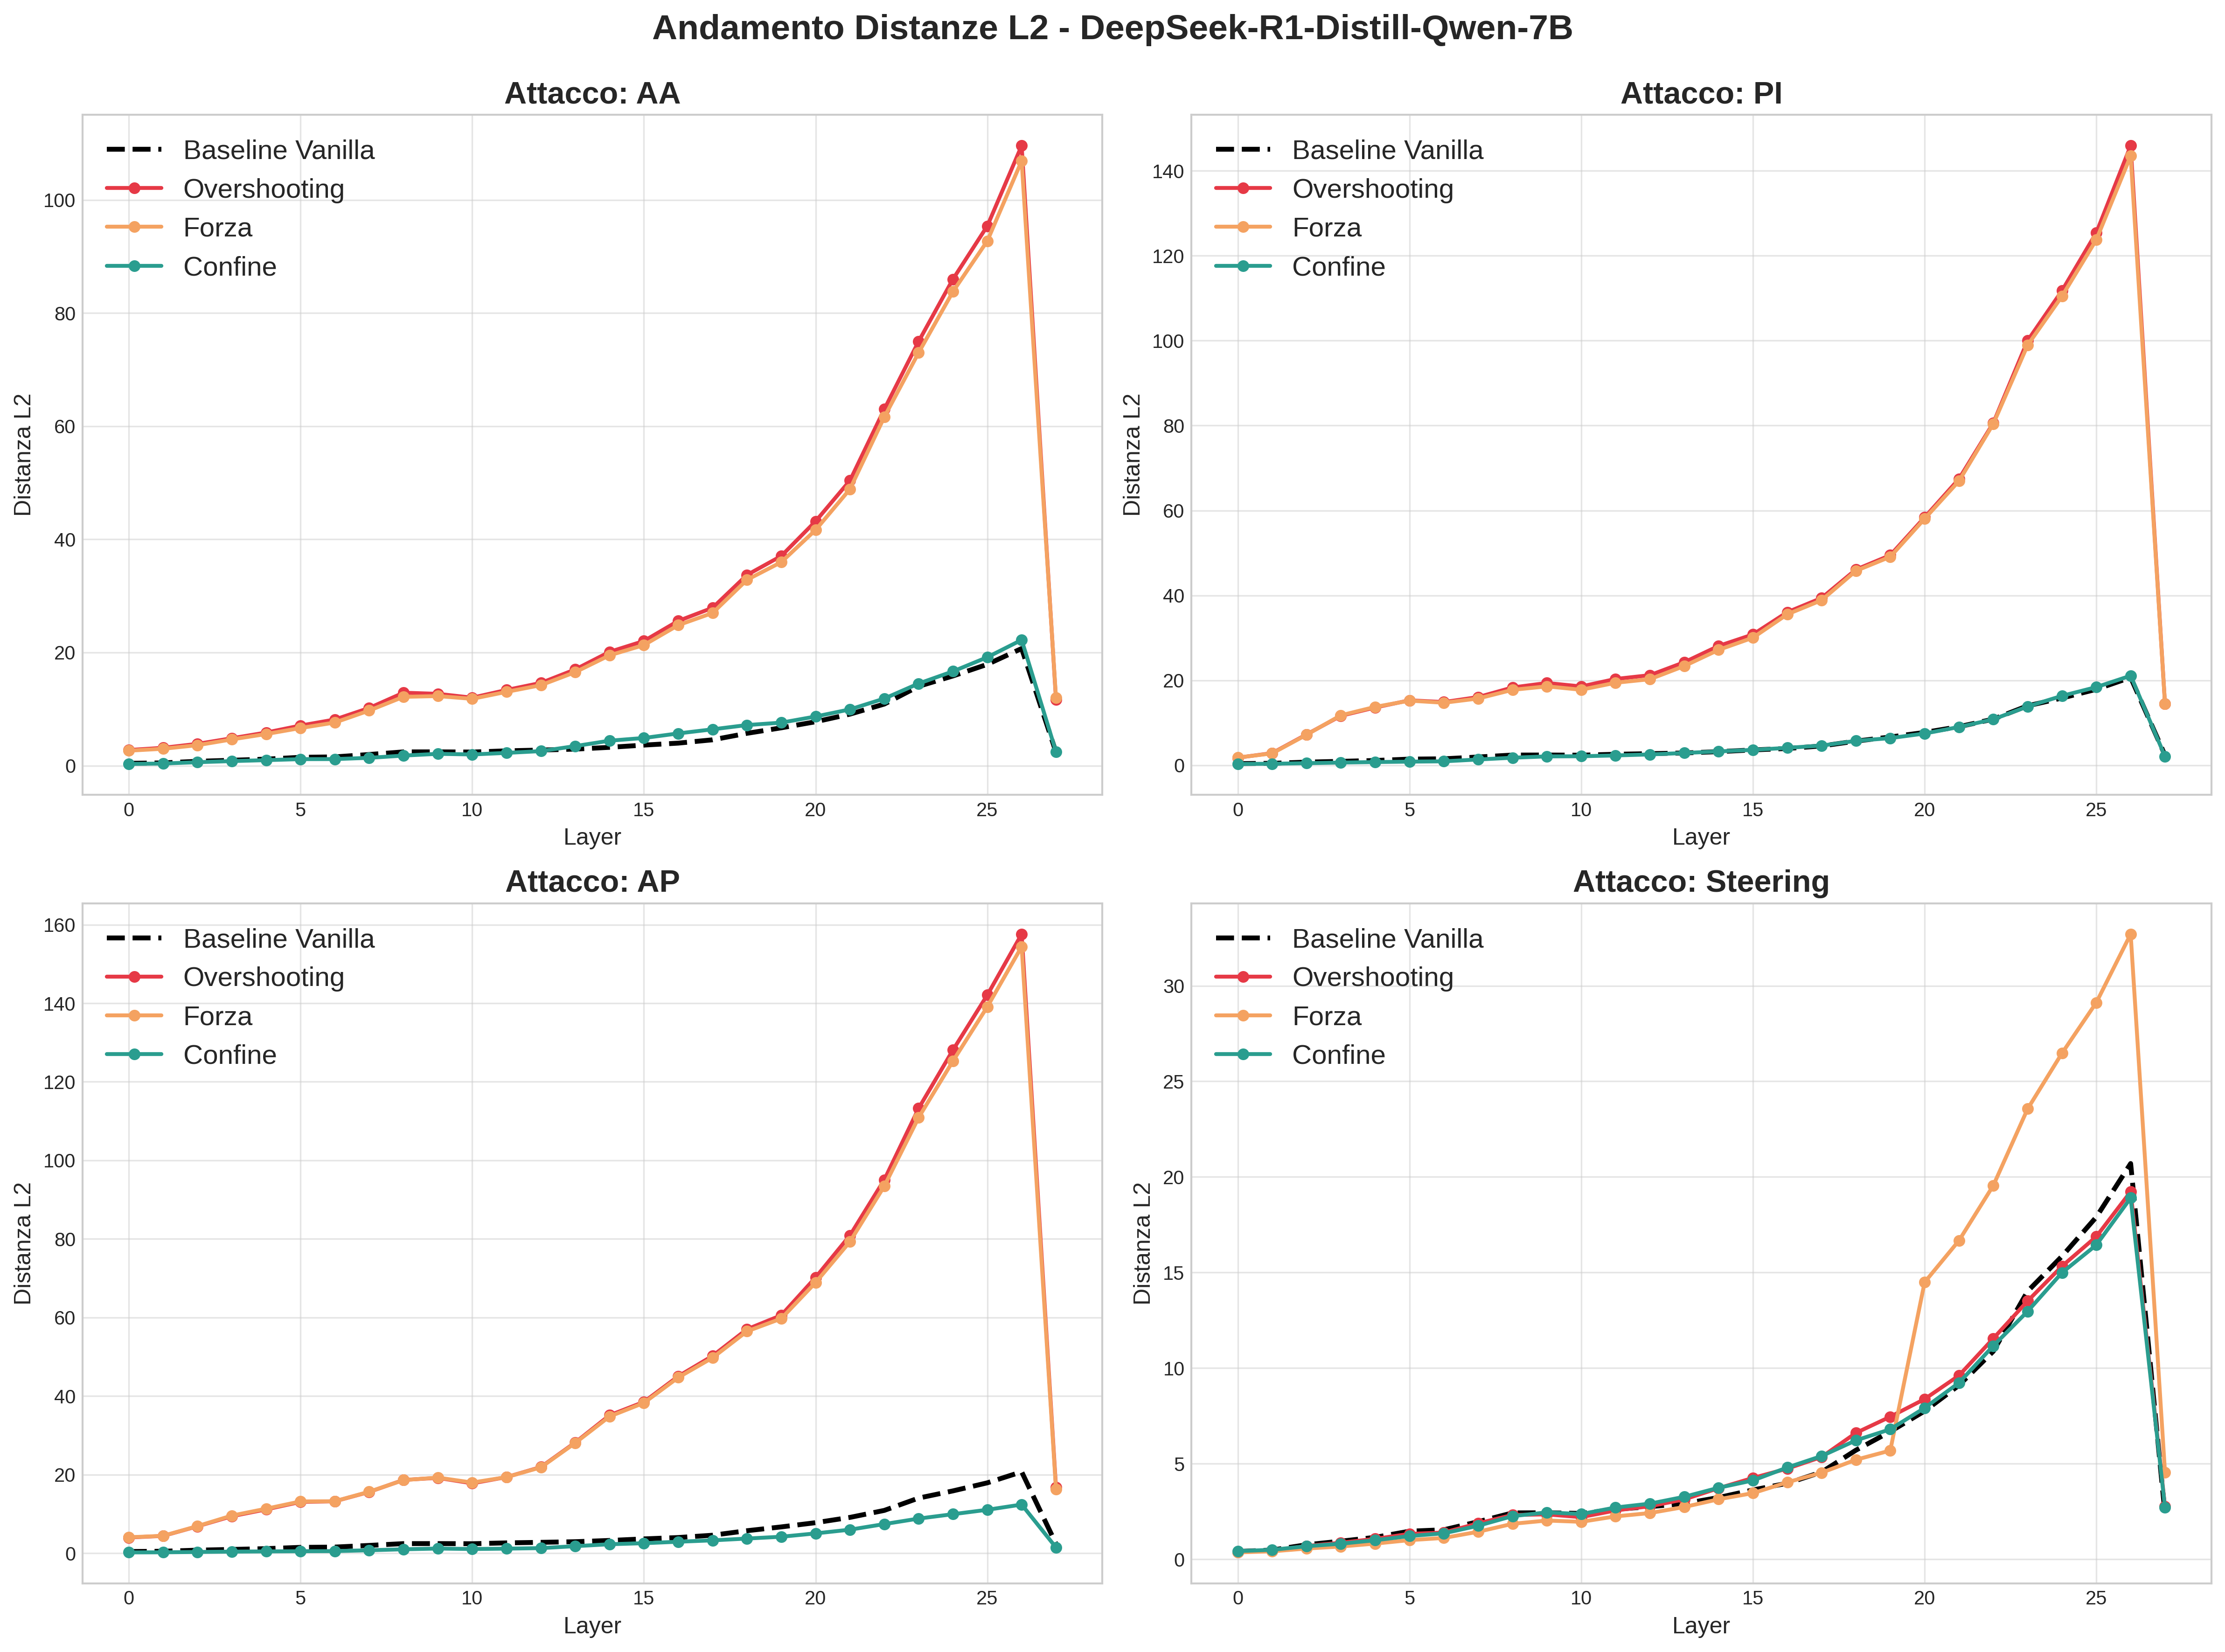
\includegraphics[width=\textwidth]{immagini/anda/DeepSeek-R1-Distill-Qwen-7B_L2_Trends.png}
\end{figure}

\begin{figure}[H]
    \centering
    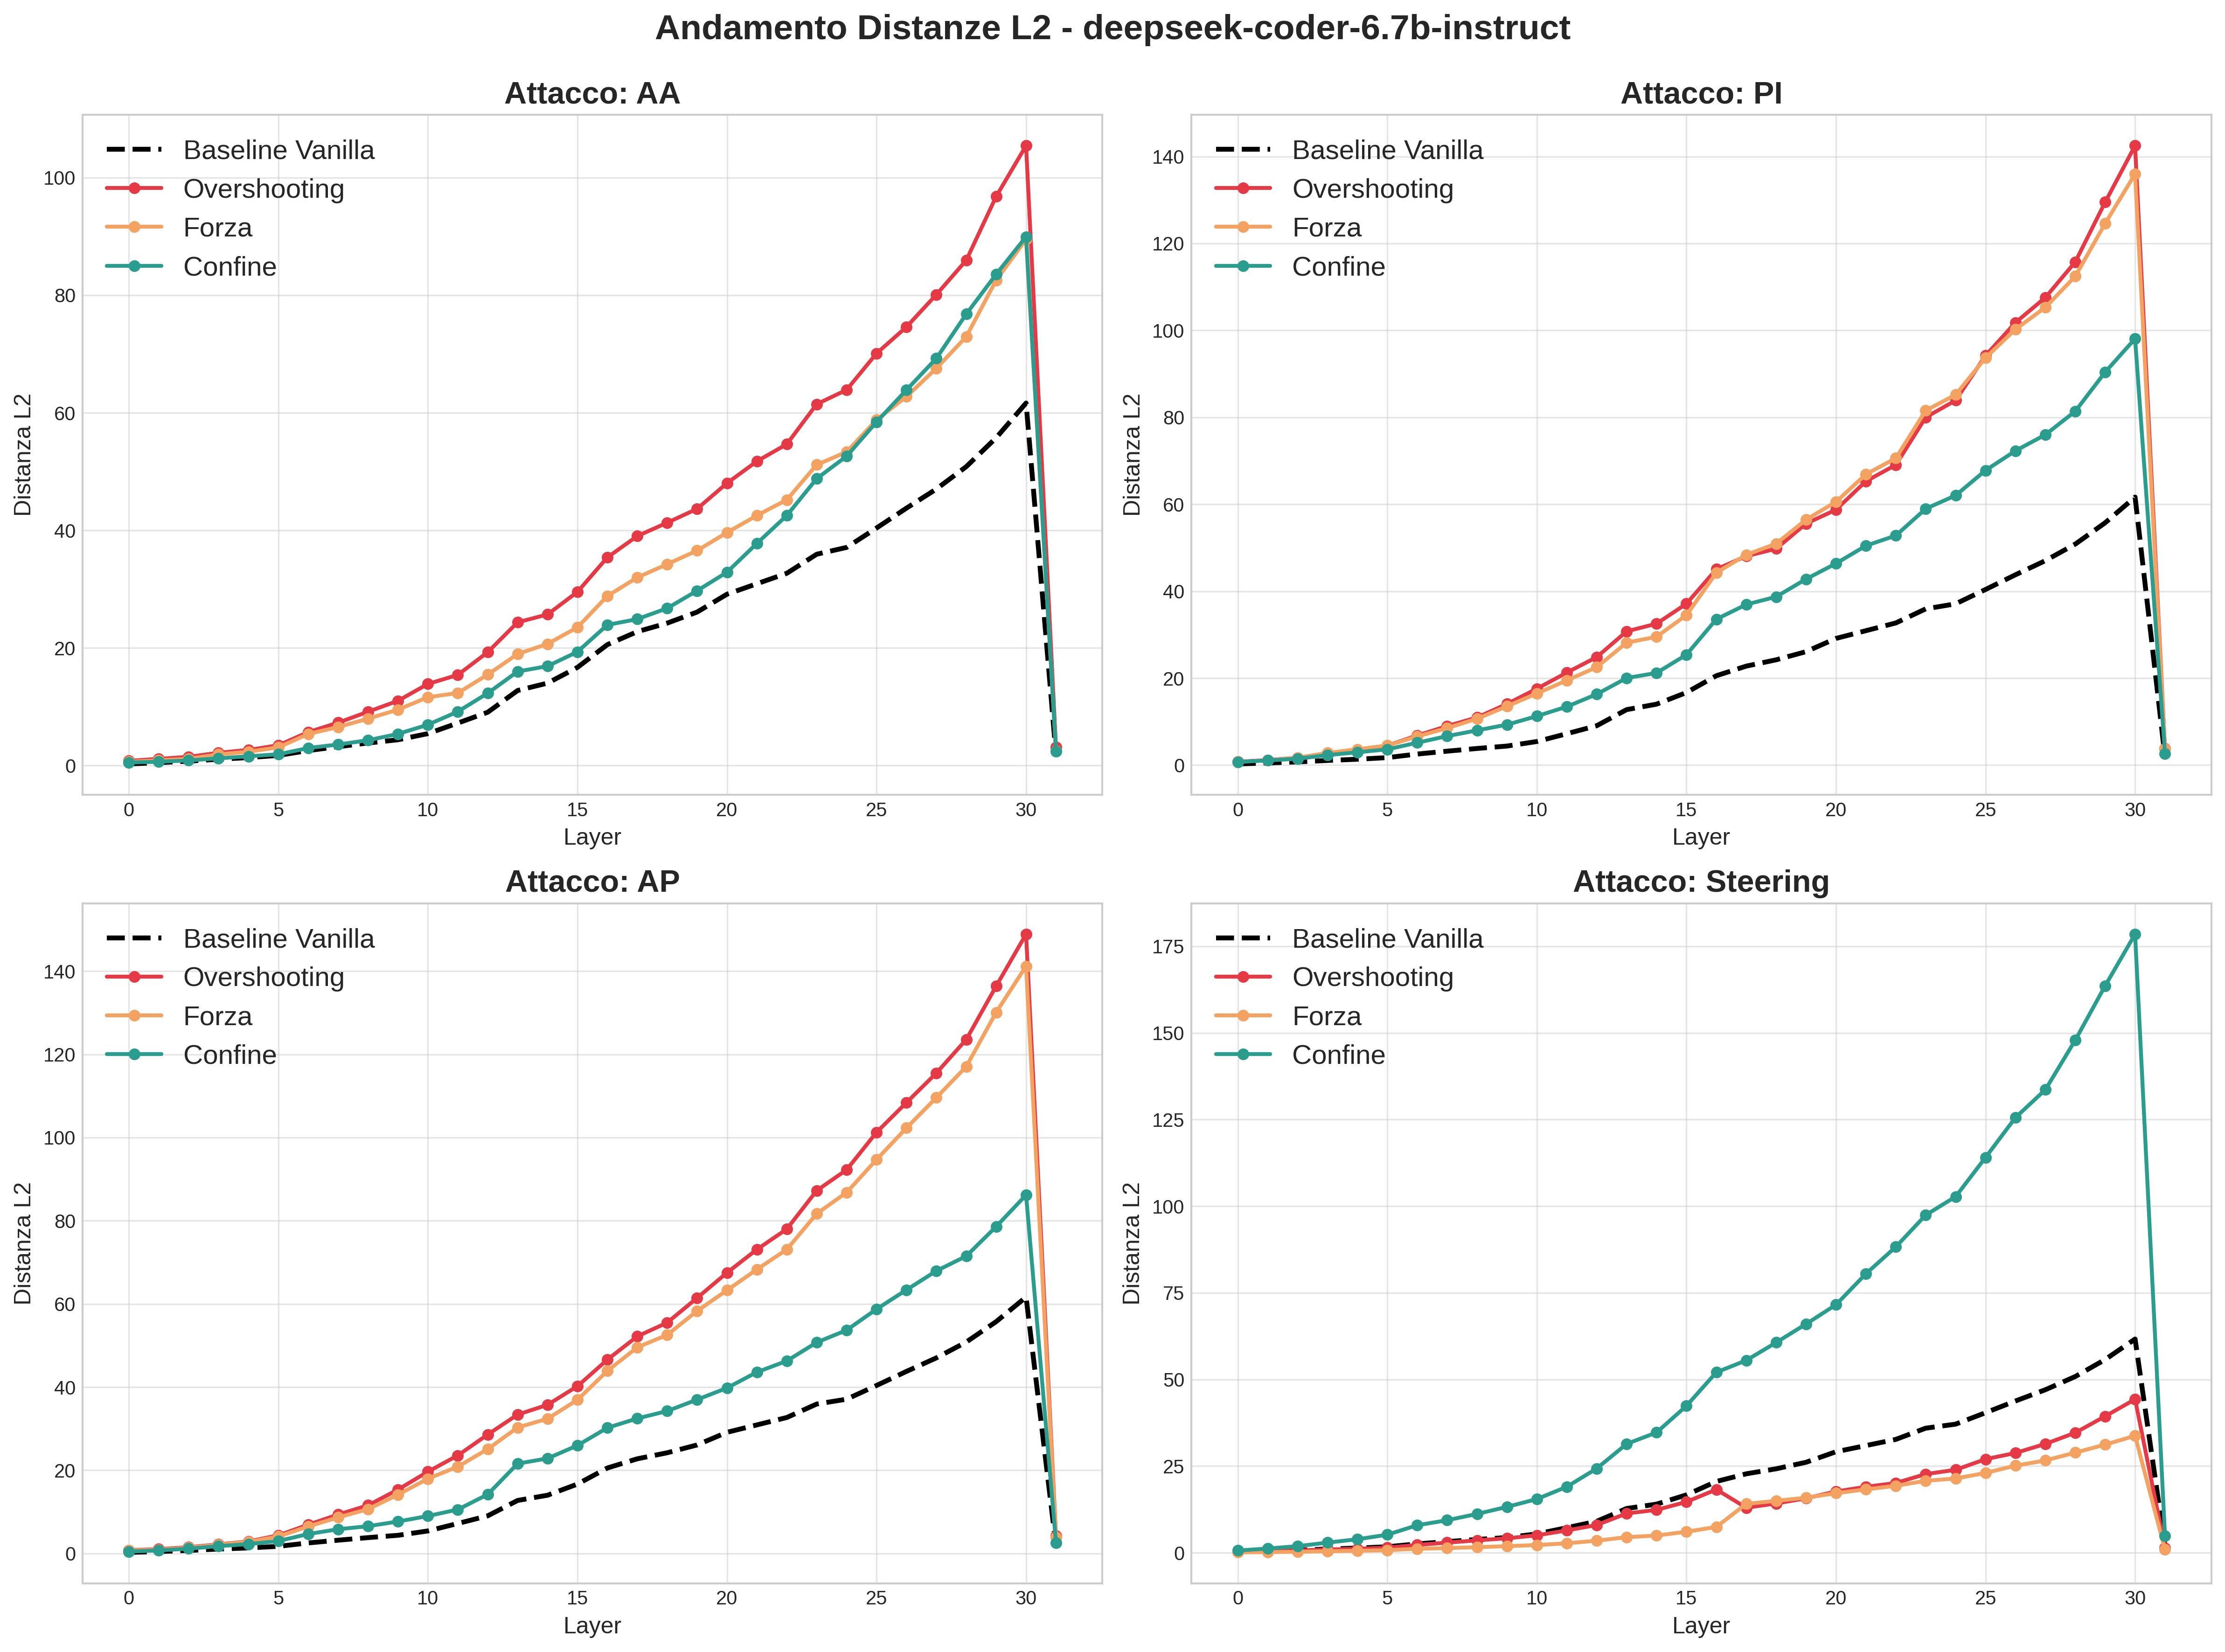
\includegraphics[width=\textwidth]{immagini/anda/deepseek-coder-6.7b-instruct_L2_Trends.png}
\end{figure}